\section{Resultados e Discussão}\label{sec:resultados_discussao}



\subsection{Visão Geral do Corpus Científico e Evolução Bibliométrica}\label{visao-geral-do-corpus-cientifico-e-evolucao-bibliometrica}

A Tabela~\ref{tab:main_info} sintetiza os principais parâmetros estatísticos e descritivos do conjunto de dados atualizado, composto por 192 documentos recuperados e validados por pares na base de dados \emph{Web of Science} (WoS). O escopo temporal foi delimitado a partir de 2004, marco histórico da introdução formal do conceito de Ligas de Alta Entropia (HEAs). Observa-se uma taxa de crescimento anual composta (CAGR) robusta de 15.76\%, evidenciando a maturidade acelerada do campo, impulsionada pelo interesse estratégico em formulações refratárias e resistência a ambientes extremos.

\begin{table}[!htbp]
\centering
\caption{Informações Principais sobre o Conjunto de Dados Analisado (2004--2026)}\label{tab:main_info}
\small
\begin{tabularx}{\textwidth}{>{\raggedright\arraybackslash}X>{\raggedright\arraybackslash}X}
\toprule
\textbf{Descrição do Indicador Bibliométrico} & \textbf{Resultado Atualizado} \\
\midrule
Período Temporal Analisado & 2004 -- 2026 \\
Total de Documentos Recuperados & 192 \\
Taxa de Crescimento Anual Composta (CAGR) & 15.76\% \\
Idade Média dos Documentos & 2.47 anos \\
Periódicos e Fontes de Publicação Dominantes & \emph{J. Alloys Compd.}, \emph{Surf. Coat. Technol.}, \emph{Appl. Surf. Sci.} \\
Tipologia Documental Dominante & Artigos de Pesquisa Original e Revisões \\
\bottomrule
\end{tabularx}
\legend{Fonte: Elaborado pelos autores (2026), com base em dados da \emph{Web of Science}.}
\end{table}

A distribuição temporal da produção científica, ilustrada na Figura~\ref{fig:annual_production}, evidencia uma trajetória evolutiva claramente demarcada em quatro fases. O período inicial de latência e fundações conceituais (2004--2009) reuniu quatro publicações pioneiras que estabeleceram as bases teóricas da alta entropia configuracional antes da exploração ampla de misturas refratárias. A fase subsequente de formulação das RHEAs (2010--2014) delimitou os primeiros sistemas equiatômicos de elevado ponto de fusão e a exploração exploratória de ligas multicomponentes concentradas, registrando dois artigos representativos. Em seguida, a fase de prova de conceito e mapeamento de gargalos (2015--2019), com nove artigos, iniciou a avaliação termomecânica sistemática e evidenciou vulnerabilidades críticas, como oxidação catastrófica e \emph{pesting}. Por fim, a fase de expansão exponencial e direcionamento a regimes severos (2020--2026) congregou 176 artigos, atingindo 53 publicações em 2025 e 50 registros em 2026 até o término da coleta, impulsionada pela demanda urgente de materiais estruturais para voos hipersônicos (Mach 5+), escudos de reentrada e sistemas de propulsão scramjet.

\begin{figure}[!htbp]
\centering
\caption{Evolução da produção científica anual (2004--2026) no corpus consolidado de 192 documentos.}\label{fig:annual_production}
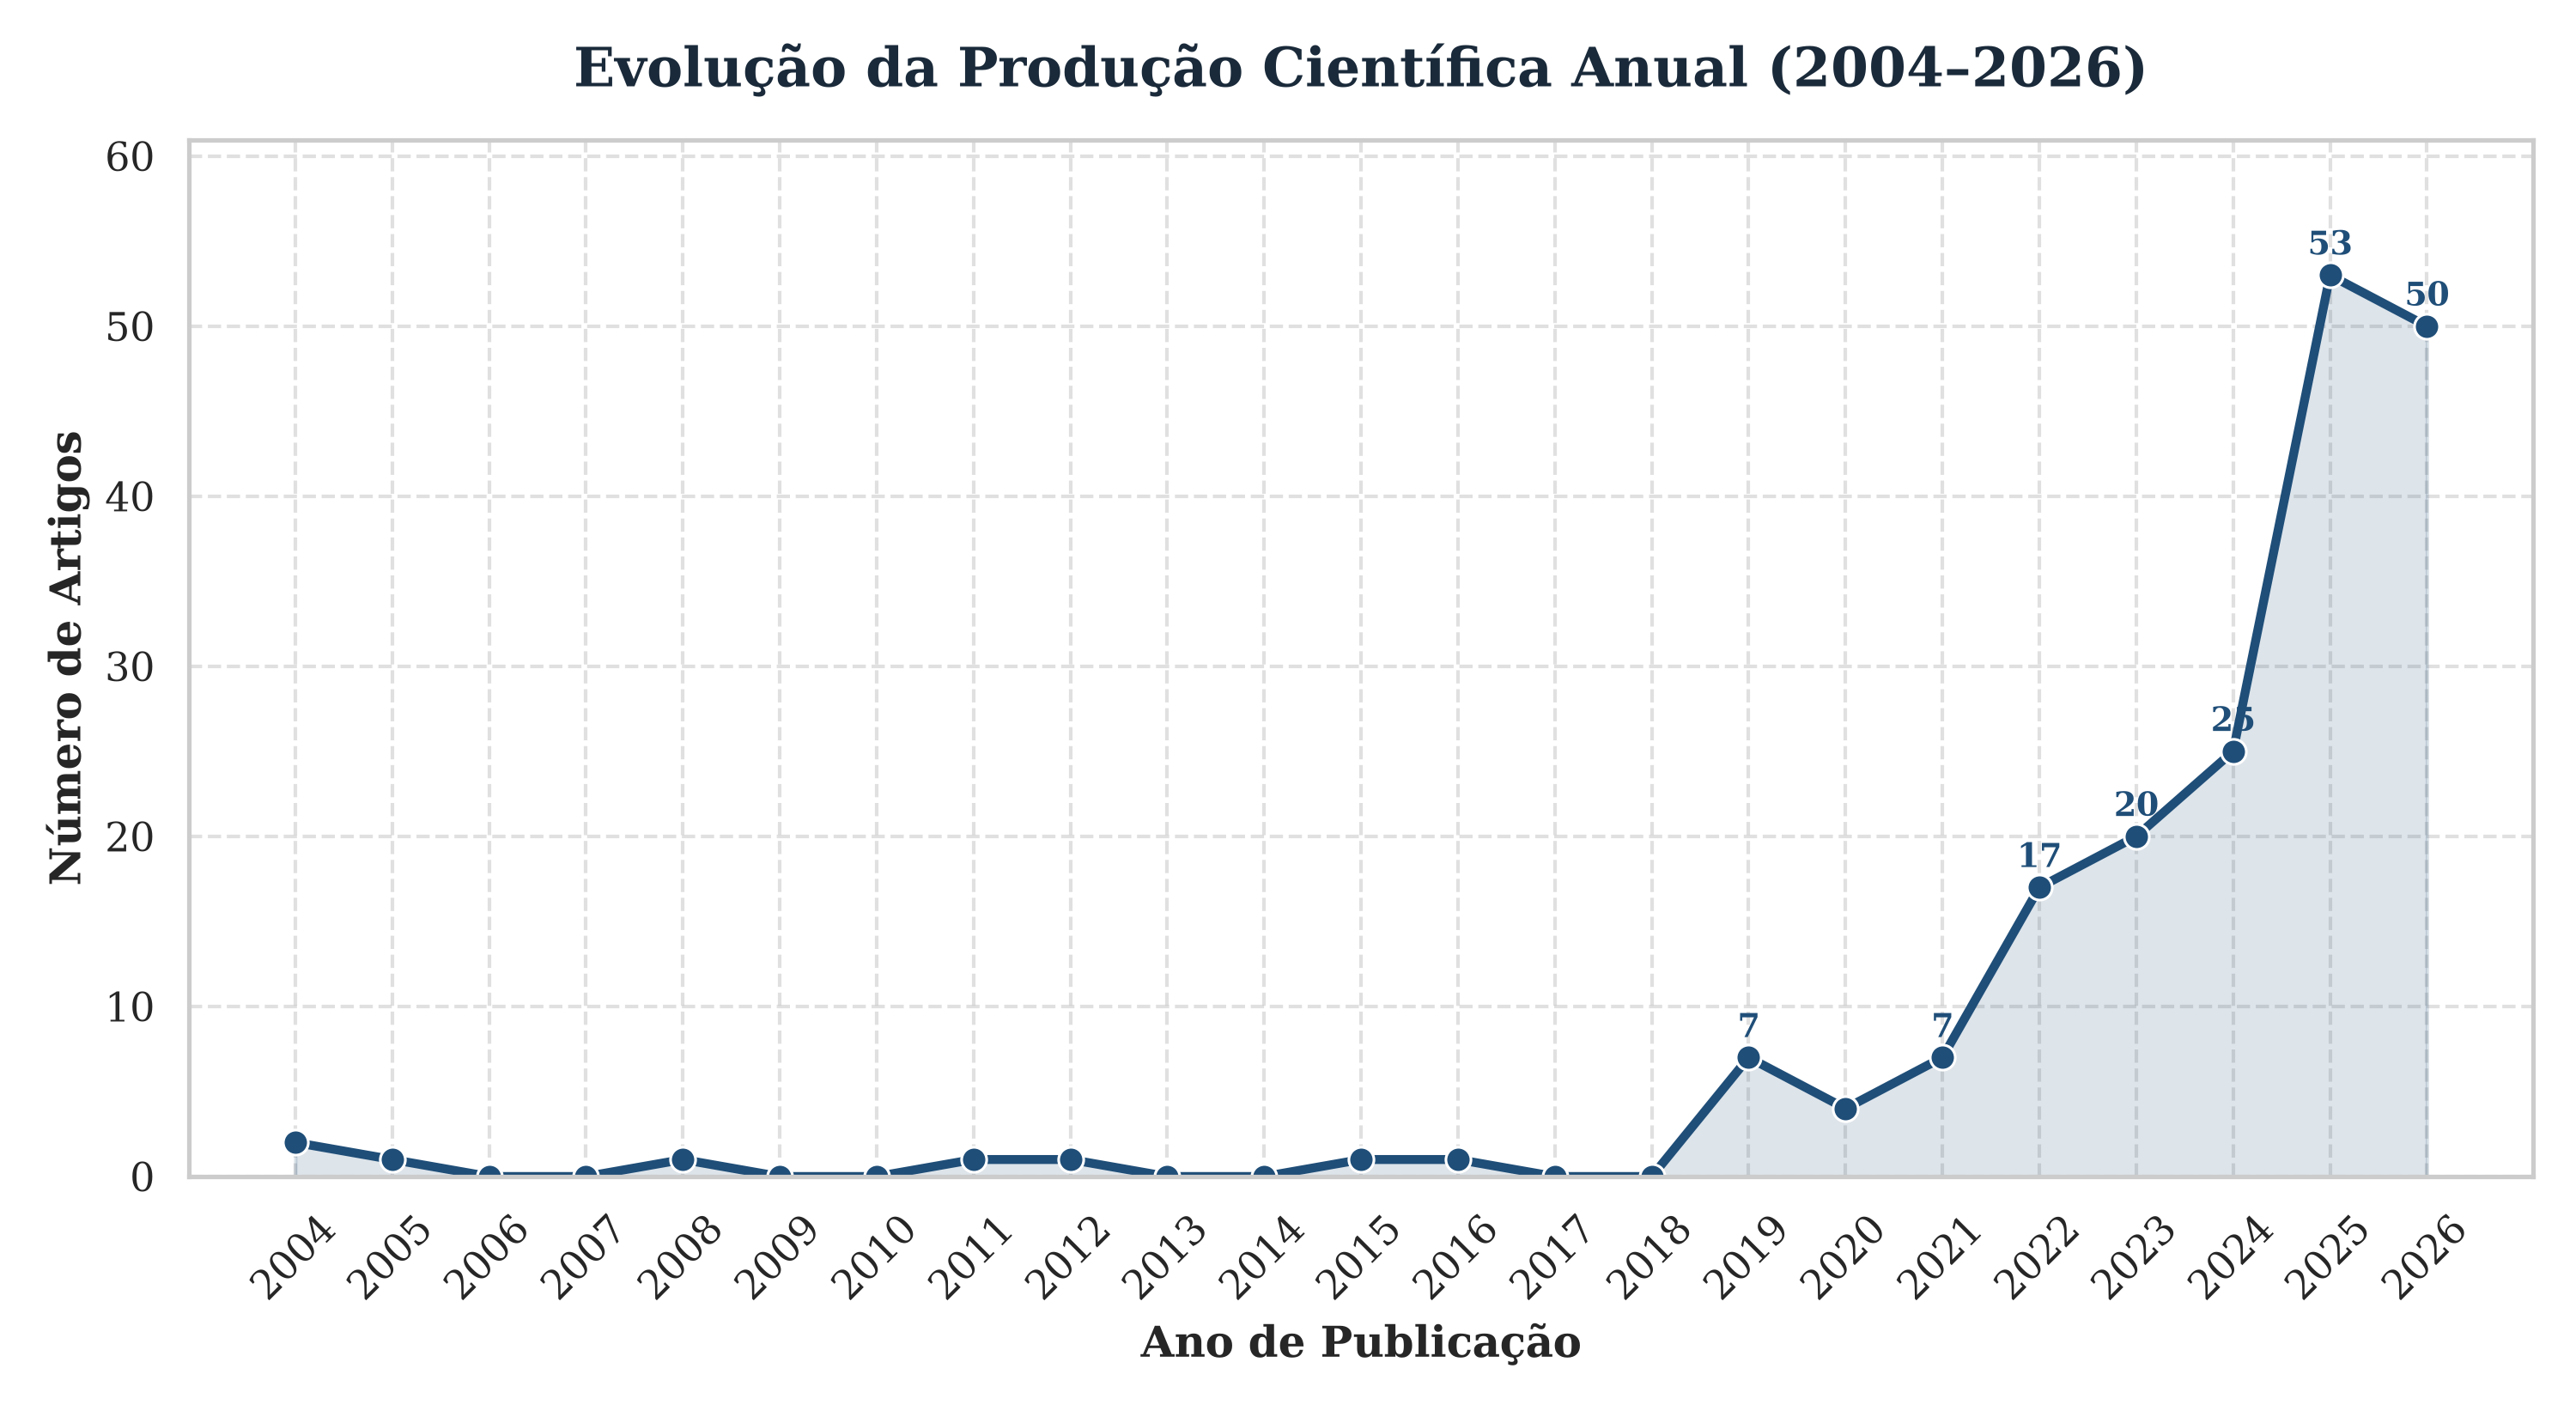
\includegraphics[width=0.85\textwidth]{figuras/annual_production.png}
\legend{Fonte: Elaborado pelos autores (2026), a partir de dados da \emph{Web of Science}.}
\end{figure}

\subsection{Perfil das Fontes de Publicação e Impacto Periódico}\label{perfil-das-fontes-de-publicacao-e-impacto-periodico}

O mapeamento das fontes de disseminação científica revela forte concentração em periódicos de alto impacto focados em física de superfícies, ciência dos materiais e revestimentos funcionais. A Figura~\ref{fig:relevant_sources} destaca as revistas científicas mais relevantes por volume de documentos publicados, lideradas pelo \emph{Journal of Alloys and Compounds} (12 artigos), seguido por \emph{Surface \& Coatings Technology} (7 artigos) e \emph{Applied Surface Science} (6 artigos), acompanhados por revistas de alto prestígio como \emph{Advanced Materials} (5 artigos) e \emph{Intermetallics} (5 artigos).

\begin{figure}[!htbp]
\centering
\caption{Periódicos mais relevantes em número absoluto de artigos publicados no corpus.}\label{fig:relevant_sources}
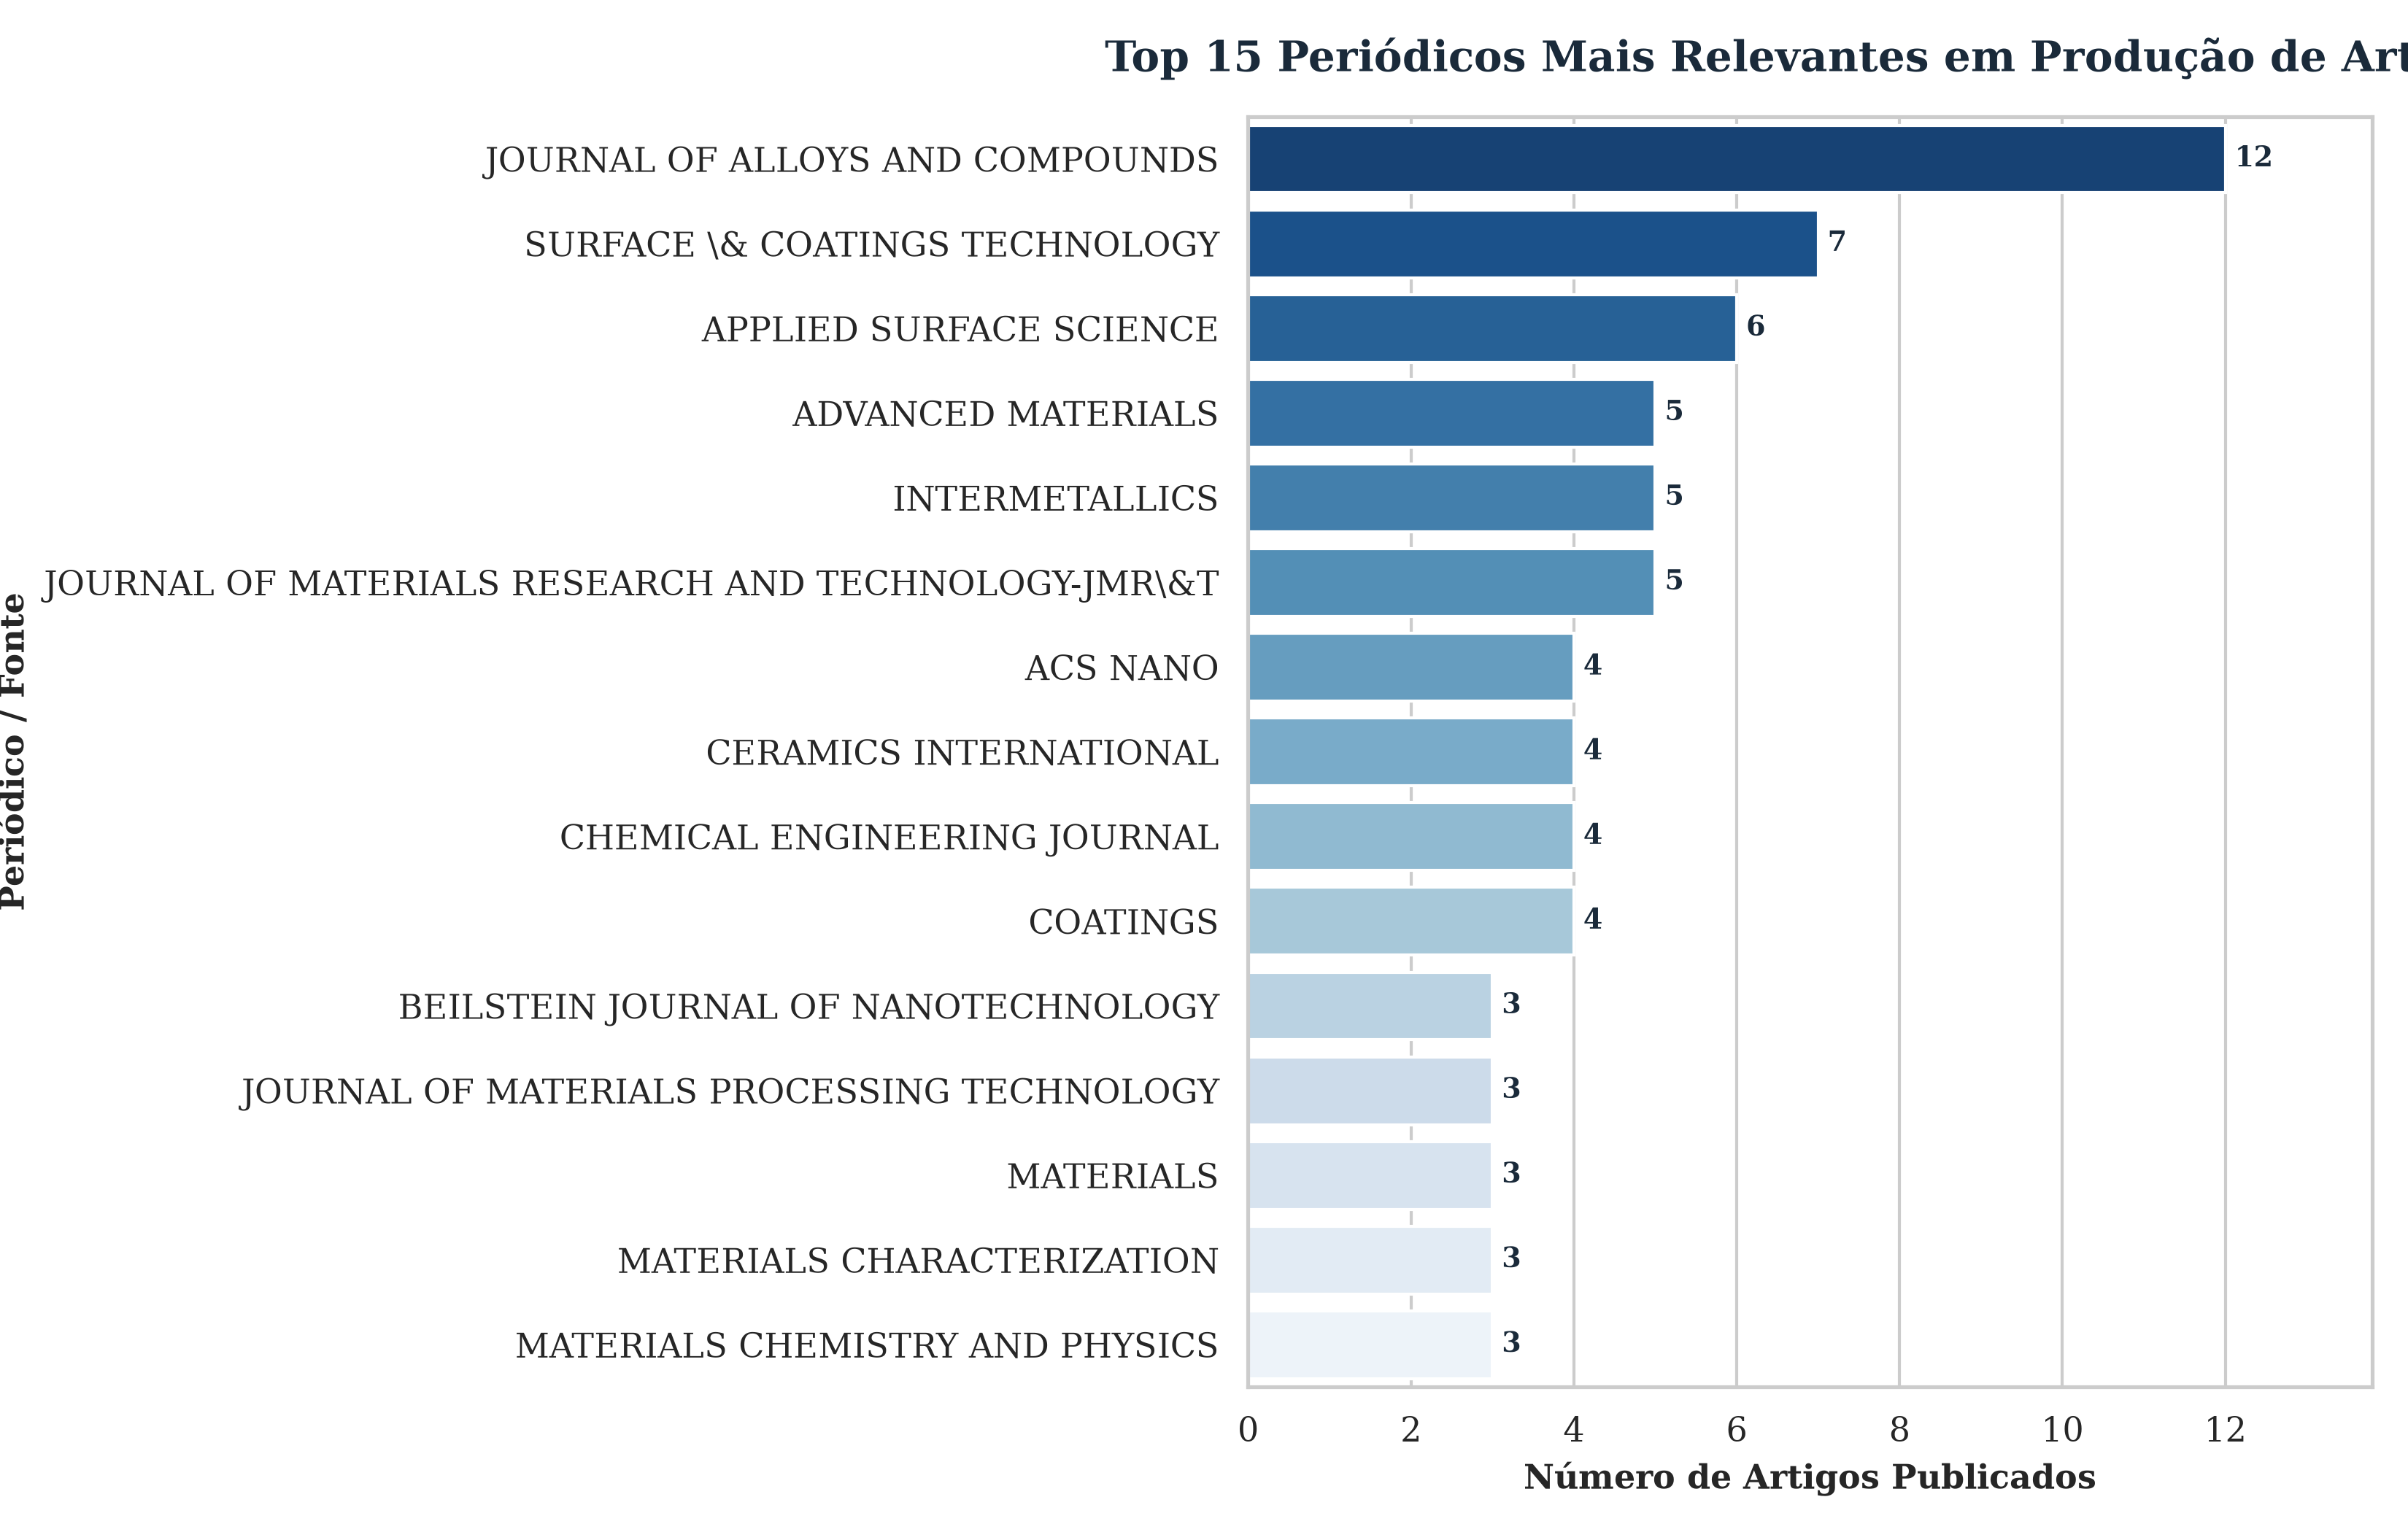
\includegraphics[width=0.85\textwidth]{figuras/most_relevant_sources.png}
\legend{Fonte: Elaborado pelos autores (2026), a partir de dados da \emph{Web of Science}.}
\end{figure}


Complementarmente, a Figura~\ref{fig:local_sources} ilustra as fontes mais citadas localmente (\emph{Local Cited Sources}), ou seja, os periódicos cujos artigos fundamentam teoricamente as pesquisas internas do corpus de 192 documentos. O \emph{Journal of Alloys and Compounds} lidera com 423 citações locais, seguido por \emph{Acta Materialia} (331 citações) e \emph{Nature Communications} (271 citações), reafirmando a convergência entre caracterização microestrutural avançada e resistência a solicitações extremas.

\begin{figure}[!htbp]
\centering
\caption{Fontes de publicação mais citadas no conjunto de referências internas do corpus.}\label{fig:local_sources}
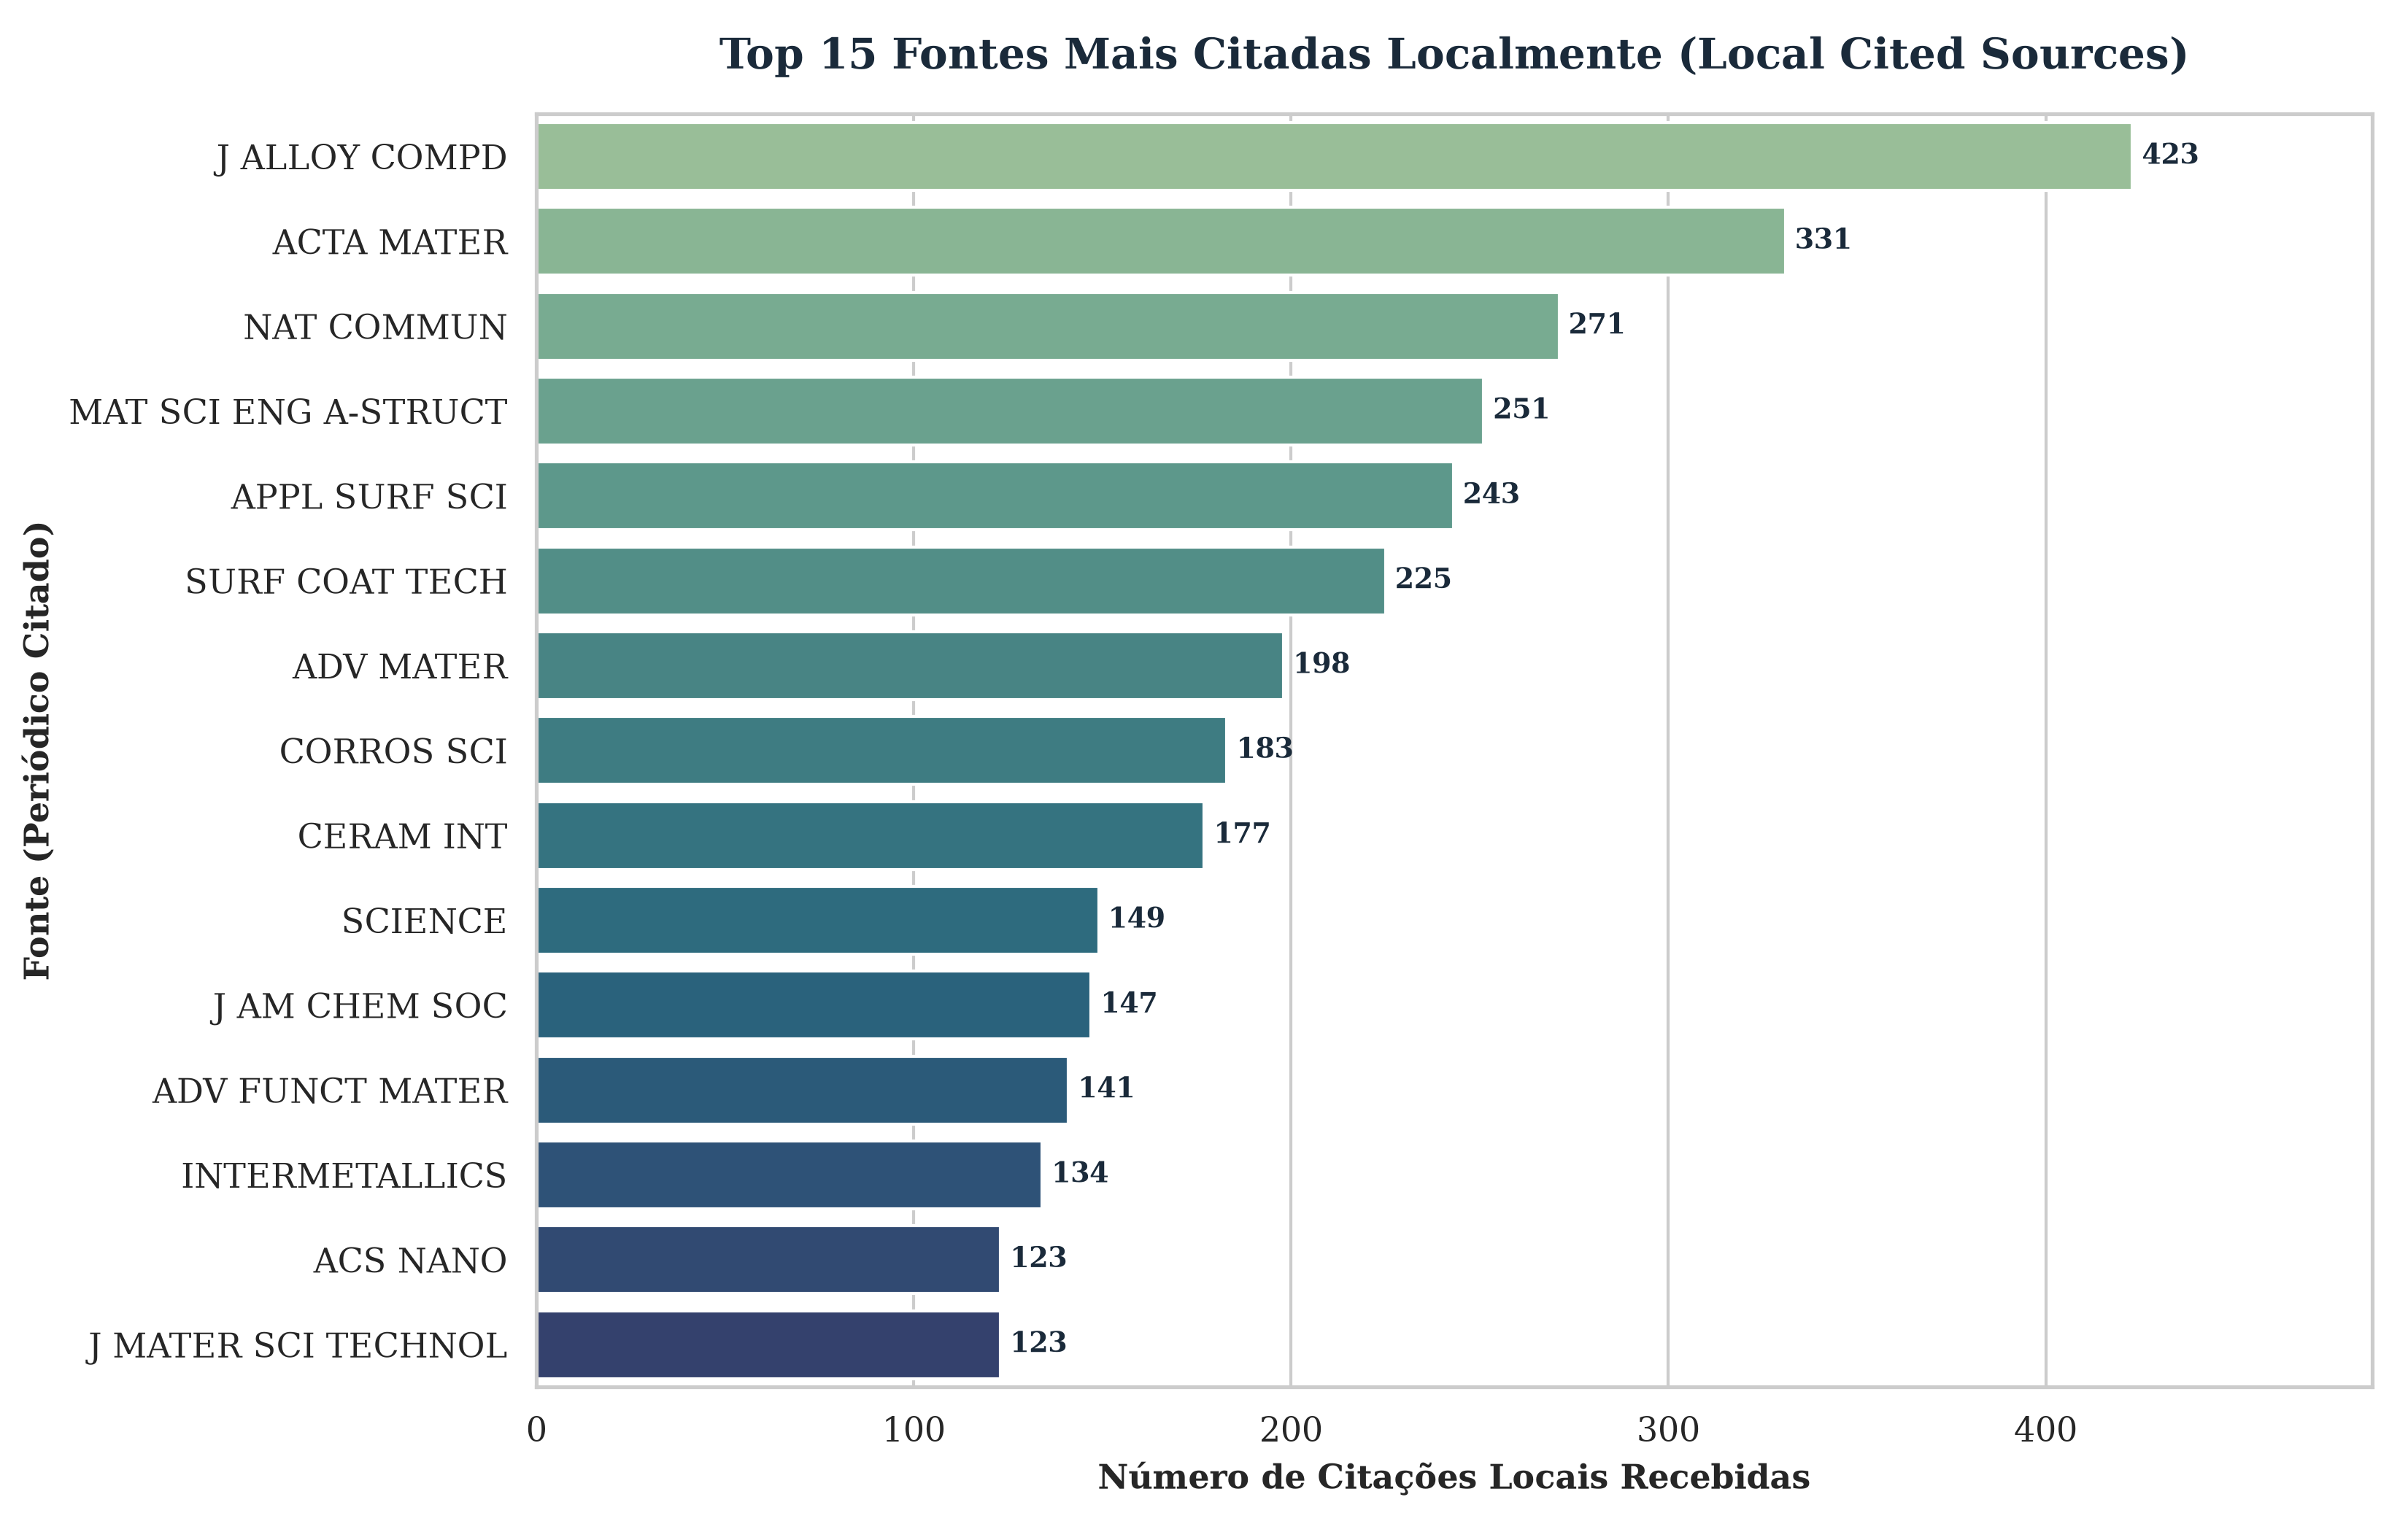
\includegraphics[width=0.85\textwidth]{figuras/most_local_cited_sources.png}
\legend{Fonte: Elaborado pelos autores (2026), a partir de dados da \emph{Web of Science}.}
\end{figure}

\subsection{Arquitetura Autoral, Institucional e Colaboração Geográfica}\label{arquitetura-autoral-institucional-e-colaboracao-geografica}

A análise de produtividade autoral no corpus atualizado (Figura~\ref{fig:relevant_authors} e Tabela~\ref{tab:authors_top10}) revela uma liderança marcante de centros de excelência em síntese de materiais e engenharia de superfícies. Destaca-se a forte atuação de pesquisadores da Alemanha (liderados por Stephan Barcikowski, Bilal Gökce, Lorenz Kienle e Christoph Rehbock) e de grupos internacionais de ponta em caracterização de materiais e fabricação aditiva na Ásia e América do Norte.

Sob a ótica do rigor cienciométrico, a interpretação da produtividade exige atenção crítica ao conhecido \textbf{efeito da homonímia} (\emph{Author Name Disambiguation} -- AND). Em bases de dados que indexam autores pela inicial e sobrenome, pesquisadores homônimos podem ser indevidamente agrupados. A verificação manual via identificadores persistentes (ORCID) e afiliações institucionais assegura a consistência das contribuições científicas identificadas neste mapeamento.

\begin{figure}[!htbp]
\centering
\caption{Os autores mais produtivos no corpus atualizado e auditado de 192 documentos.}\label{fig:relevant_authors}
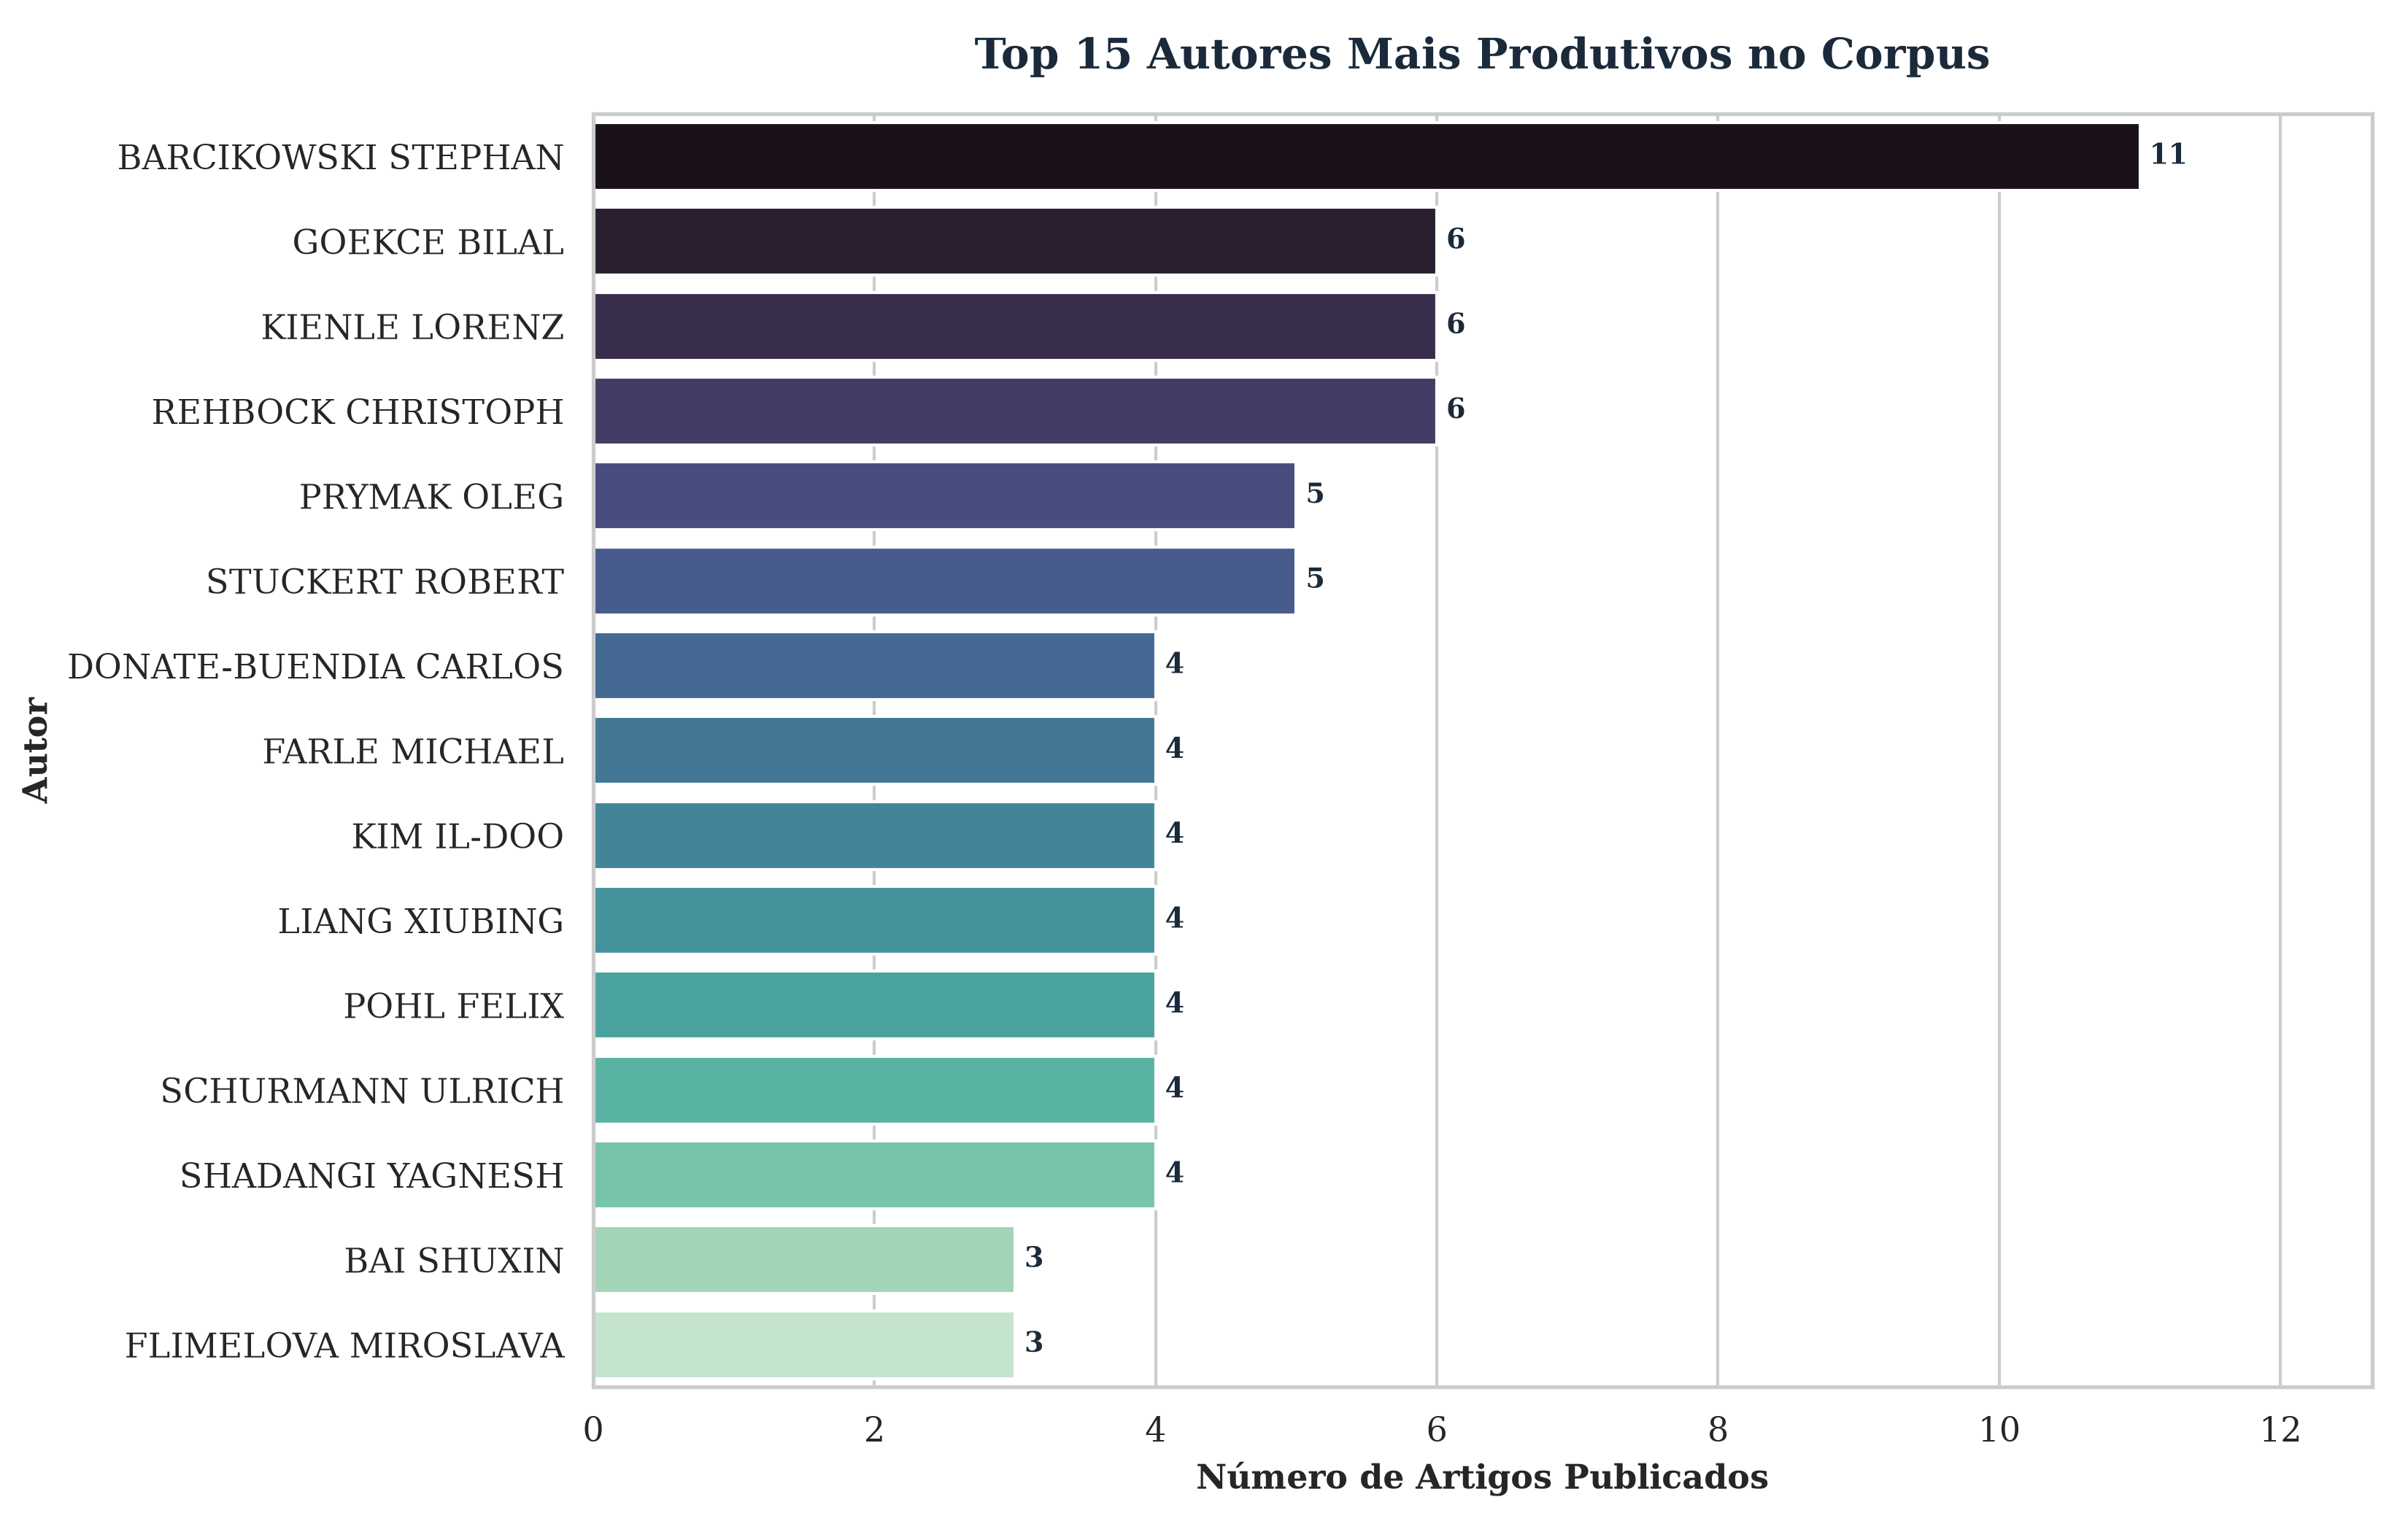
\includegraphics[width=0.85\textwidth]{figuras/most_relevant_authors.png}
\legend{Fonte: Elaborado pelos autores (2026), a partir de dados da \emph{Web of Science}.}
\end{figure}

\begin{table}[!htbp]
\centering
\caption{Os 10 Autores Mais Produtivos no Corpus e Principais Afiliações}\label{tab:authors_top10}
\small
\begin{tabularx}{\textwidth}{lc>{\raggedright\arraybackslash}X}
\toprule
\textbf{Autor} & \textbf{Artigos} & \textbf{Afiliação Institucional Dominante} \\
\midrule
BARCIKOWSKI S & 11 & University of Duisburg-Essen (Alemanha) \\
GOEKCE B & 6 & Univ. Wuppertal / Duisburg-Essen (Alemanha) \\
KIENLE L & 6 & University of Kiel (Alemanha) \\
REHBOCK C & 6 & University of Duisburg-Essen (Alemanha) \\
PRYMAK O & 5 & University of Duisburg-Essen (Alemanha) \\
STUCKERT R & 5 & University of Duisburg-Essen (Alemanha) \\
DONATE-BUENDIA C & 4 & Univ. Jaume I (Espanha) / Duisburg-Essen \\
FARLE M & 4 & University of Duisburg-Essen (Alemanha) \\
KIM ID & 4 & KAIST (Coreia do Sul) \\
LIANG XB & 4 & Academy of Armored Forces Engineering (China) \\
\bottomrule
\end{tabularx}
\legend{Fonte: Elaborado pelos autores (2026), com base em dados da \emph{Web of Science}.}
\end{table}

A distribuição das afiliações institucionais mais produtivas (Figura~\ref{fig:relevant_affiliations}) reforça esse ecossistema colaborativo. A \emph{University of Duisburg-Essen} (39 artigos) lidera o \emph{ranking} global com folga, seguida pela \emph{Shandong University} (16 artigos), \emph{University of Hyderabad} (12 artigos), \emph{Tianjin University of Technology and Education} (10 artigos) e \emph{Xi'an Jiaotong University} (10 artigos).

\begin{figure}[!htbp]
\centering
\caption{Afiliações institucionais mais produtivas no corpus de 192 documentos.}\label{fig:relevant_affiliations}
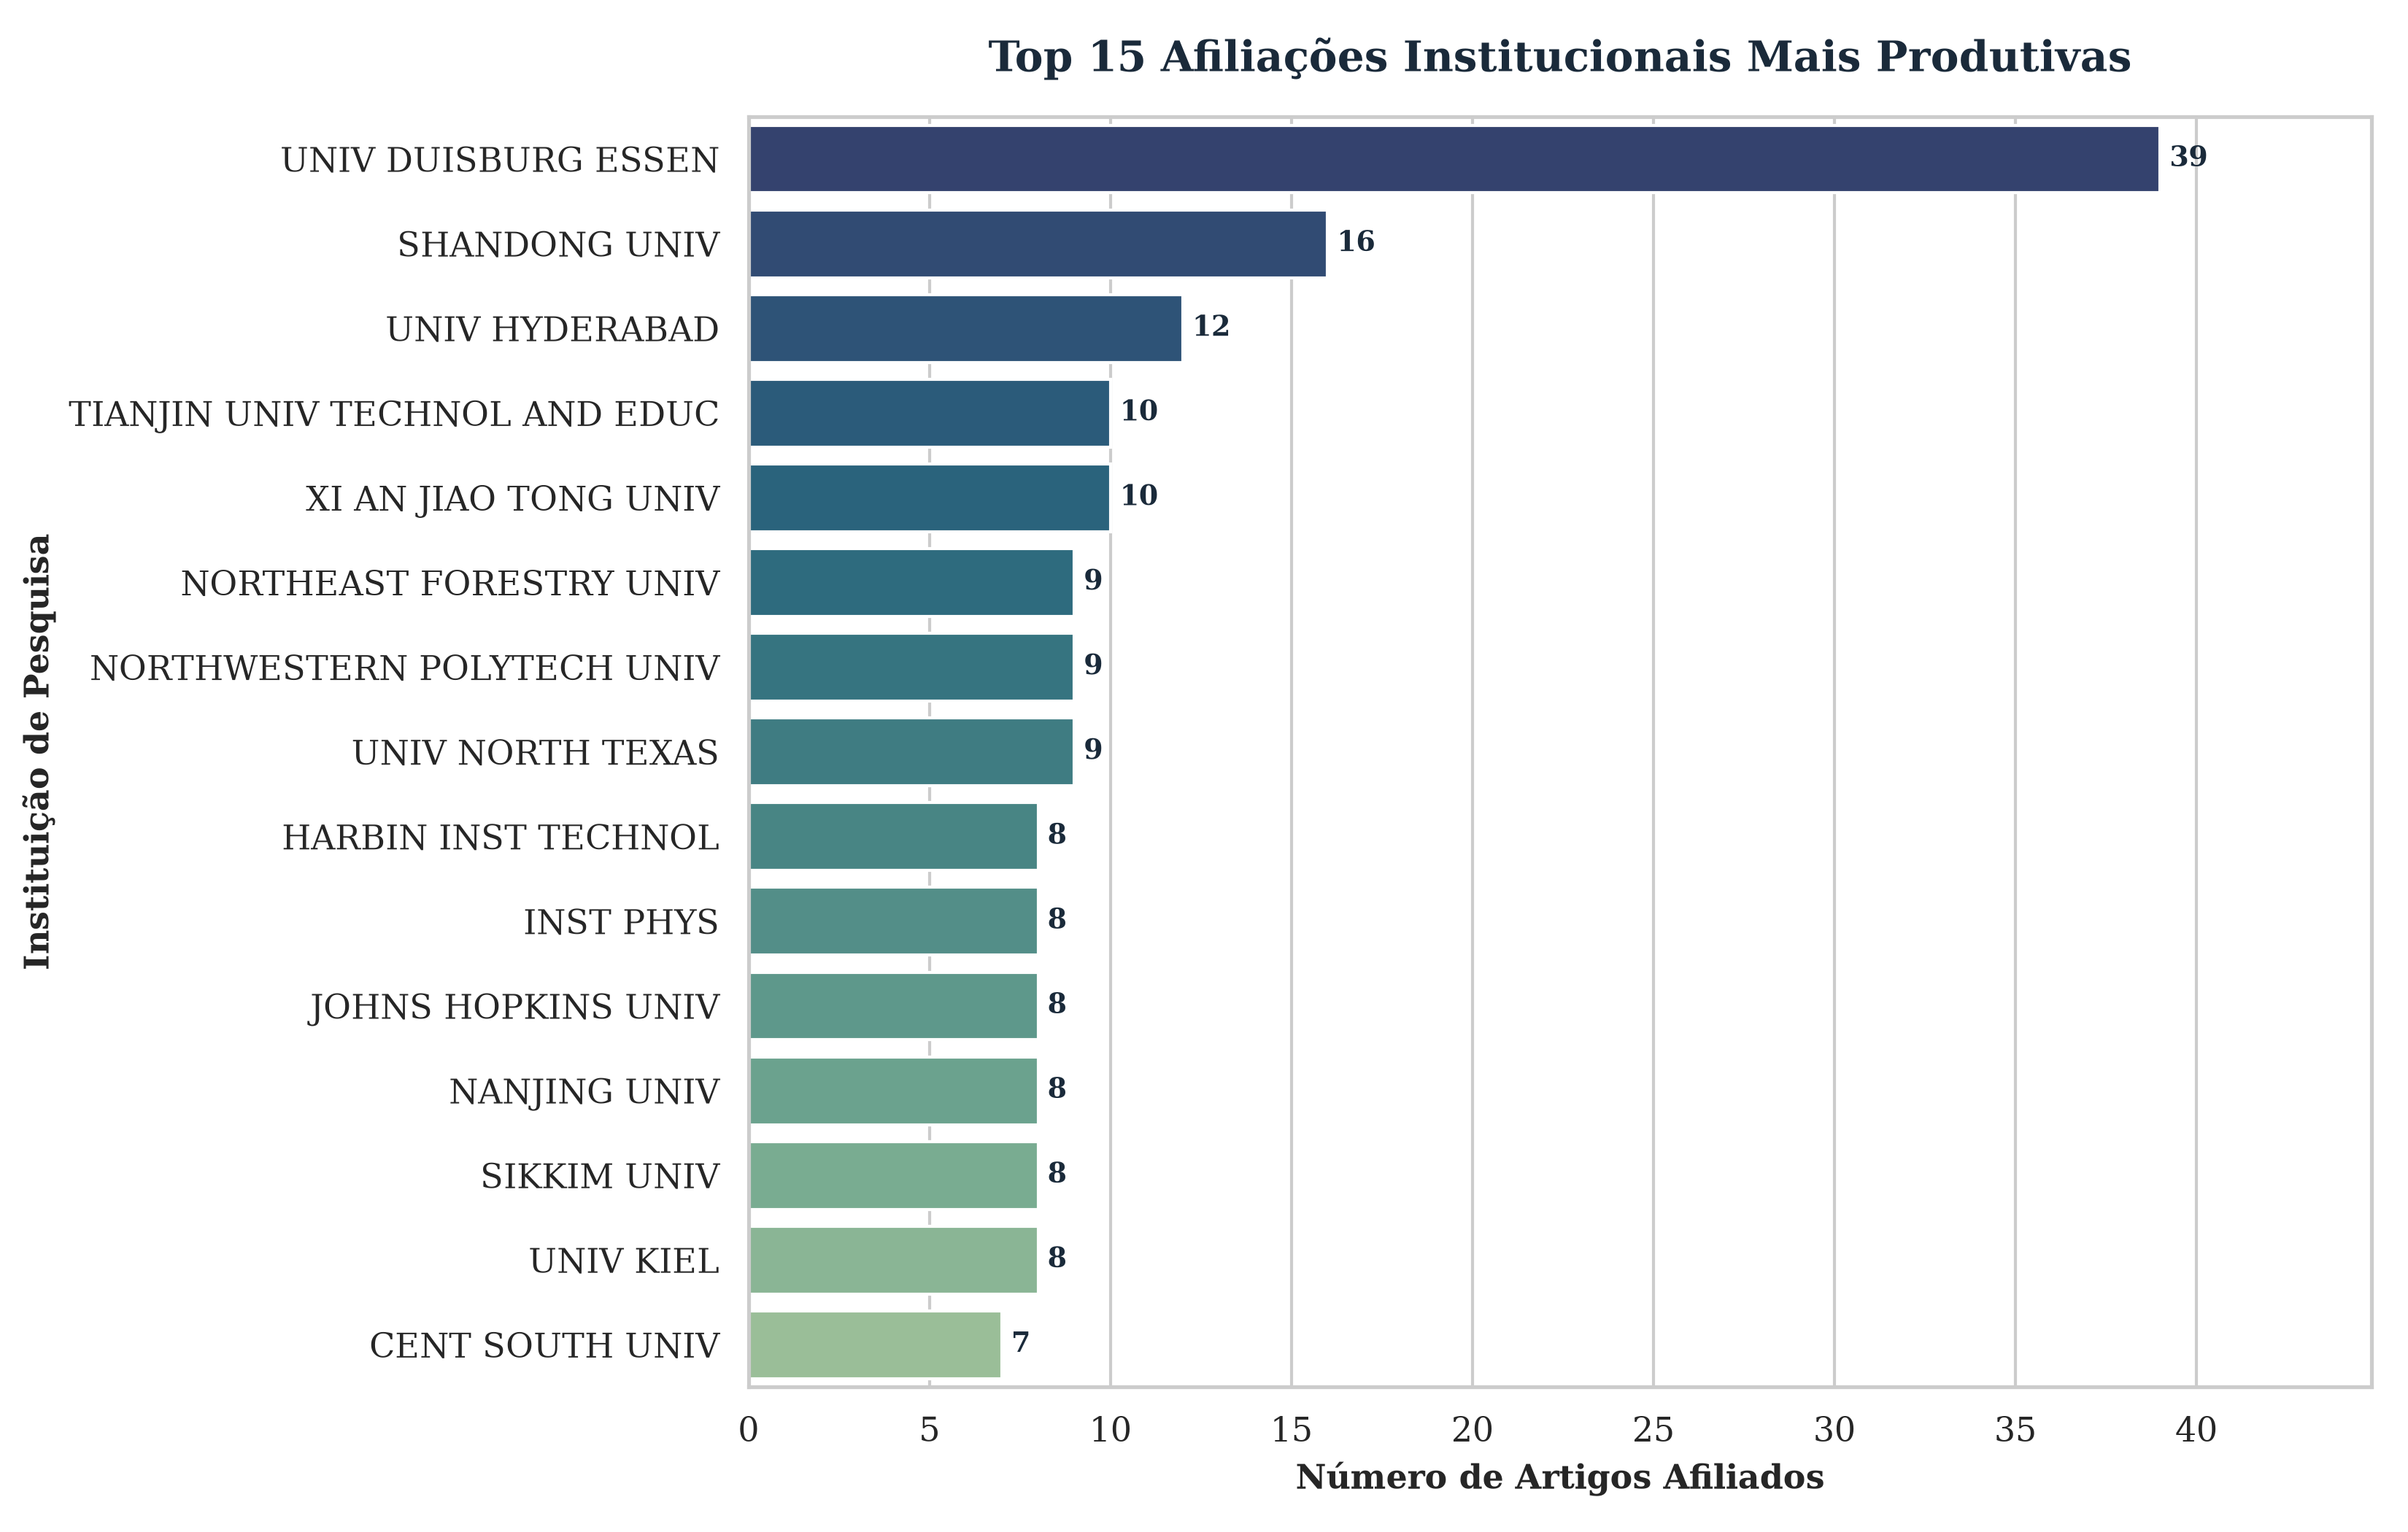
\includegraphics[width=0.85\textwidth]{figuras/most_relevant_affiliations.png}
\legend{Fonte: Elaborado pelos autores (2026), a partir de dados da \emph{Web of Science}.}
\end{figure}

A rede de colaboração internacional e cocitação, exposta na Figura~\ref{fig:collaboration_network}, demonstra agrupamentos fortemente conectados regionalmente, indicando a presença de consórcios nacionais e parcerias estratégicas de pesquisa impulsionando ligas refratárias.

\begin{figure}[!htbp]
\centering
\caption{Rede de cocitação e agrupamento intelectual construída via análise topológica (NetworkX), demonstrando centralidade e modularidade dos clusters no campo das RHEAs.}\label{fig:collaboration_network}
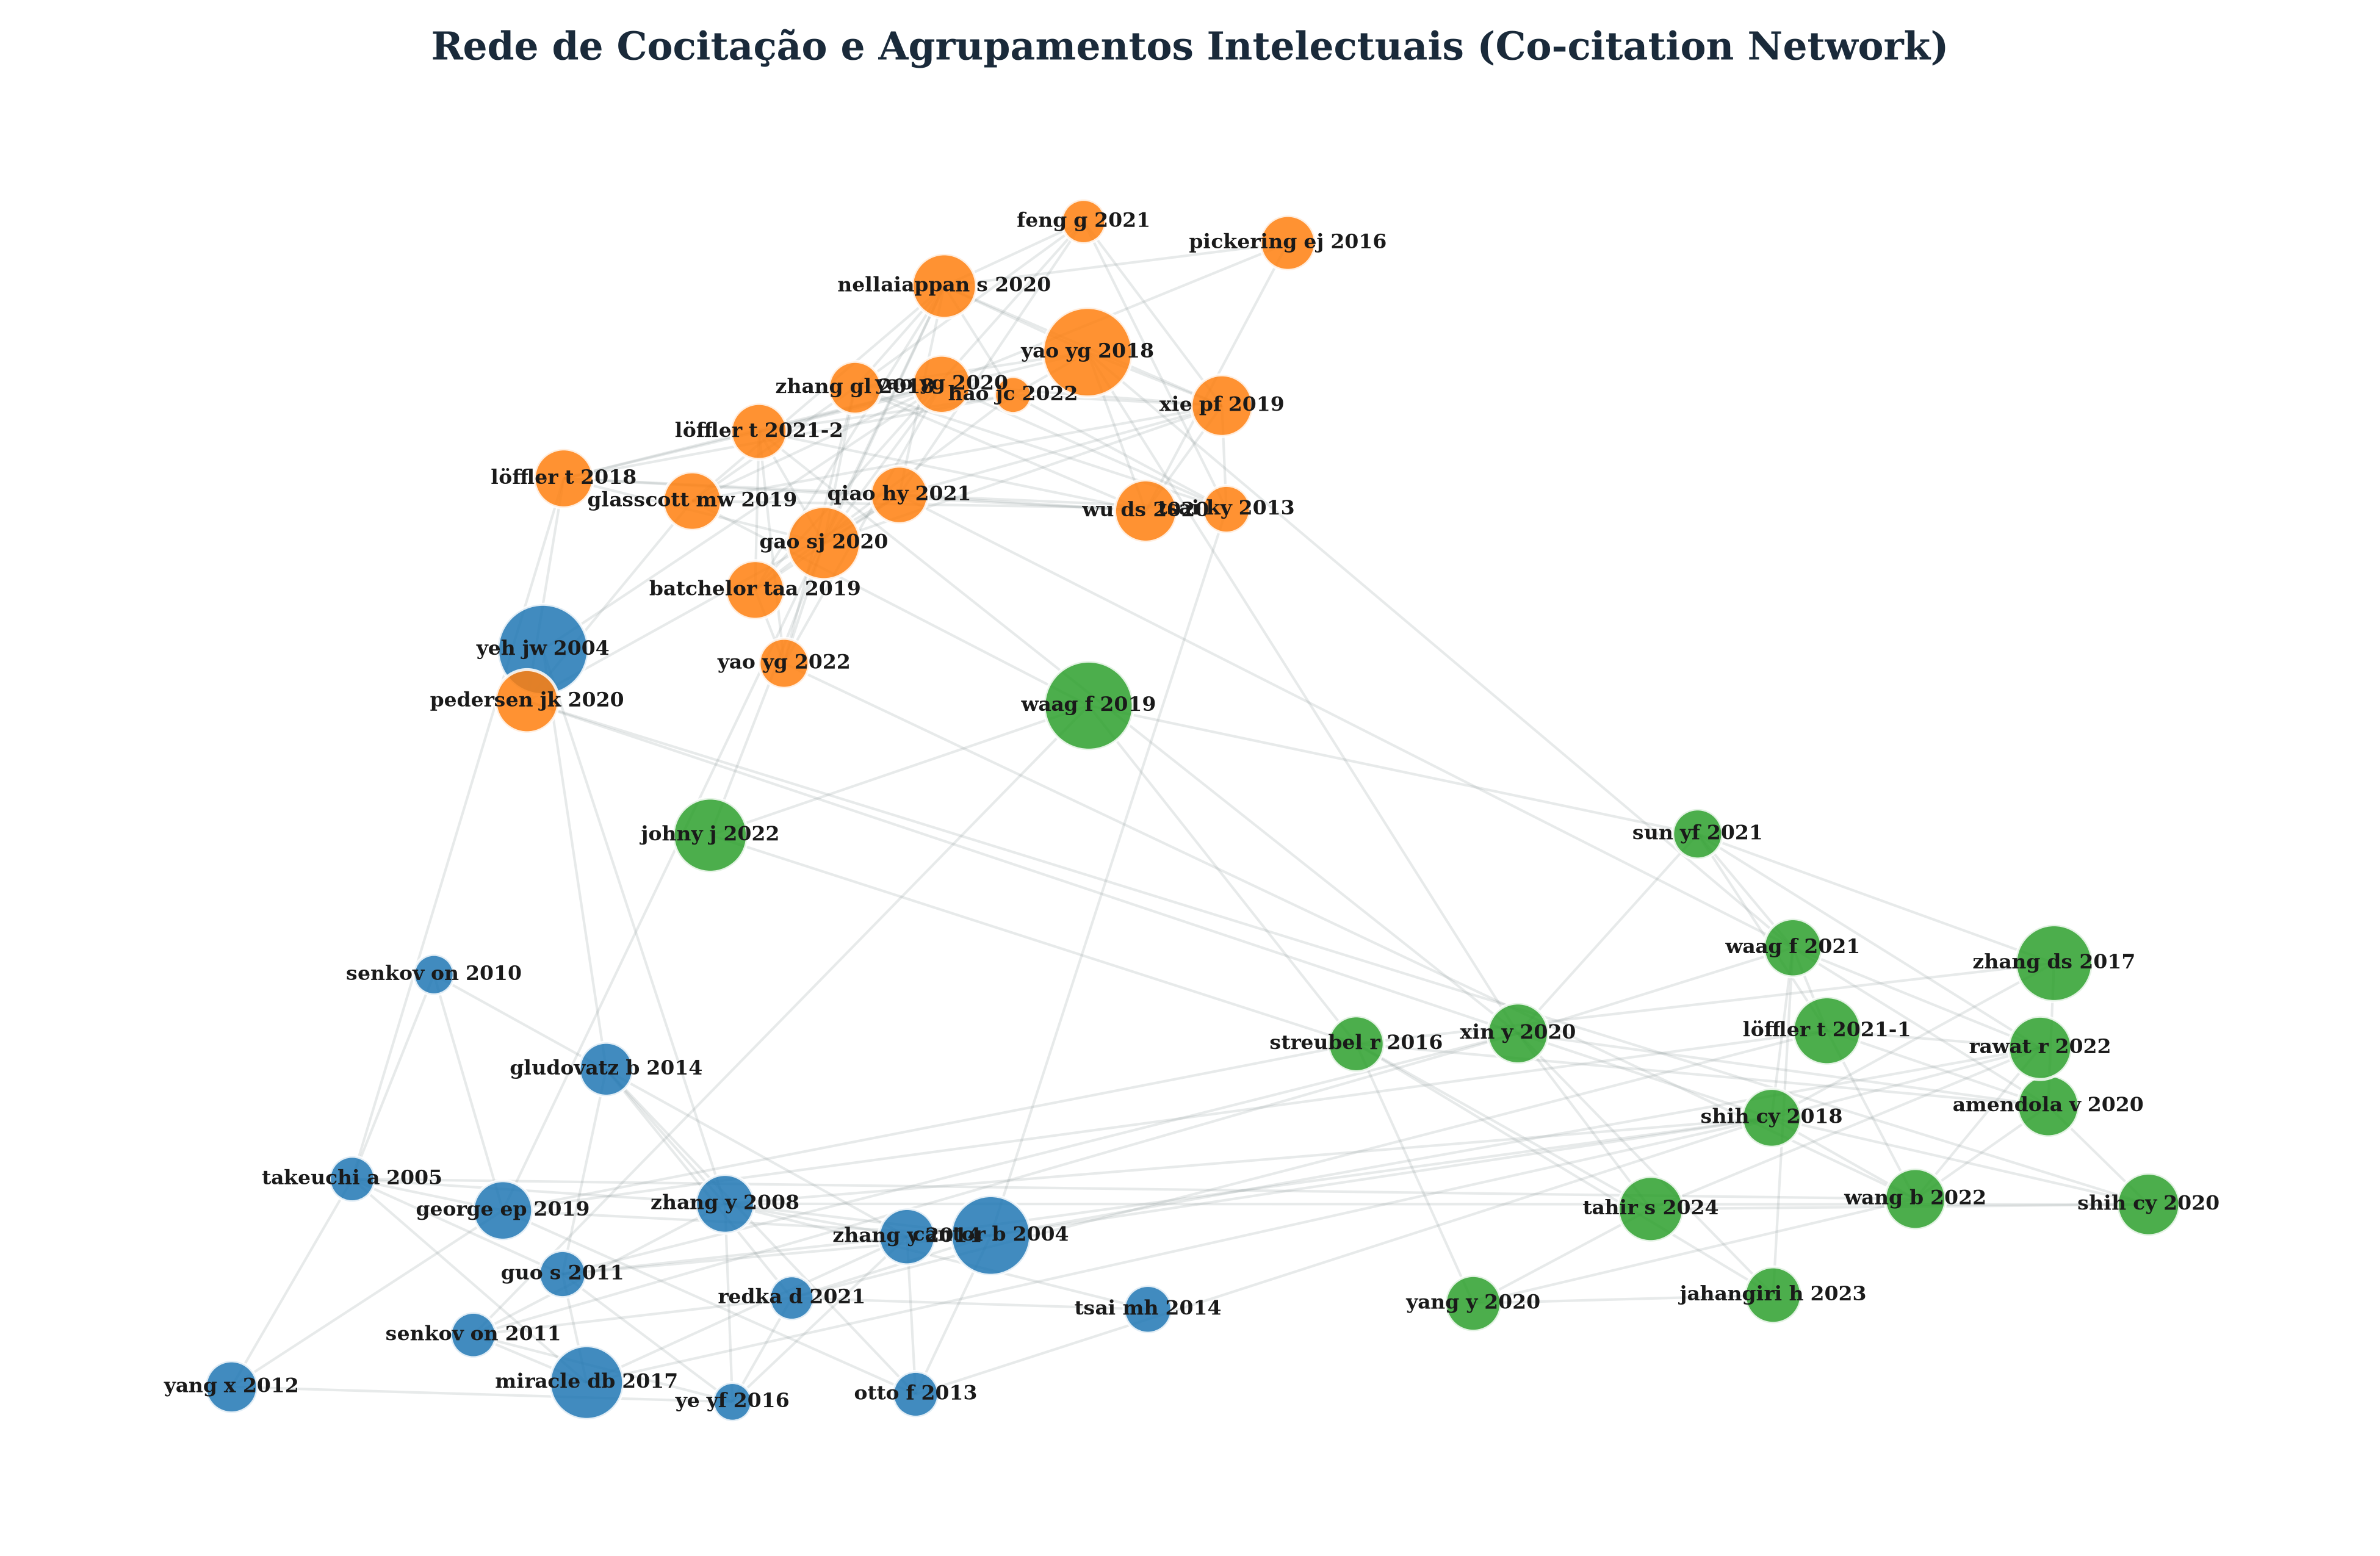
\includegraphics[width=0.85\textwidth]{figuras/cocit_network.png}
\legend{Fonte: Elaborado pelos autores (2026), a partir de dados da \emph{Web of Science}.}
\end{figure}

\subsection{Artigos Mais Citados Global e Localmente}\label{artigos-mais-citados-global-e-localmente}

O impacto das publicações no ecossistema científico global é apresentado na Figura~\ref{fig:global_cited} e sumarizado na Tabela~\ref{tab:top_glob_docs}. O estudo de Peters et al. (2024), publicado na \emph{Nature Communications}, desponta como o artigo mais citado globalmente (462 citações e notável taxa de 154 citações por ano), destacando-se na fronteira de design de materiais para aplicações hipersônicas. É seguido por Wang B. et al. (2022) na \emph{Nature Synthesis} (302 citações; 60,40 cit./ano) e por Waag et al. (2019) na \emph{RSC Advances} (242 citações).

\begin{figure}[!htbp]
\centering
\caption{Os artigos mais citados globalmente dentro do conjunto de dados.}\label{fig:global_cited}
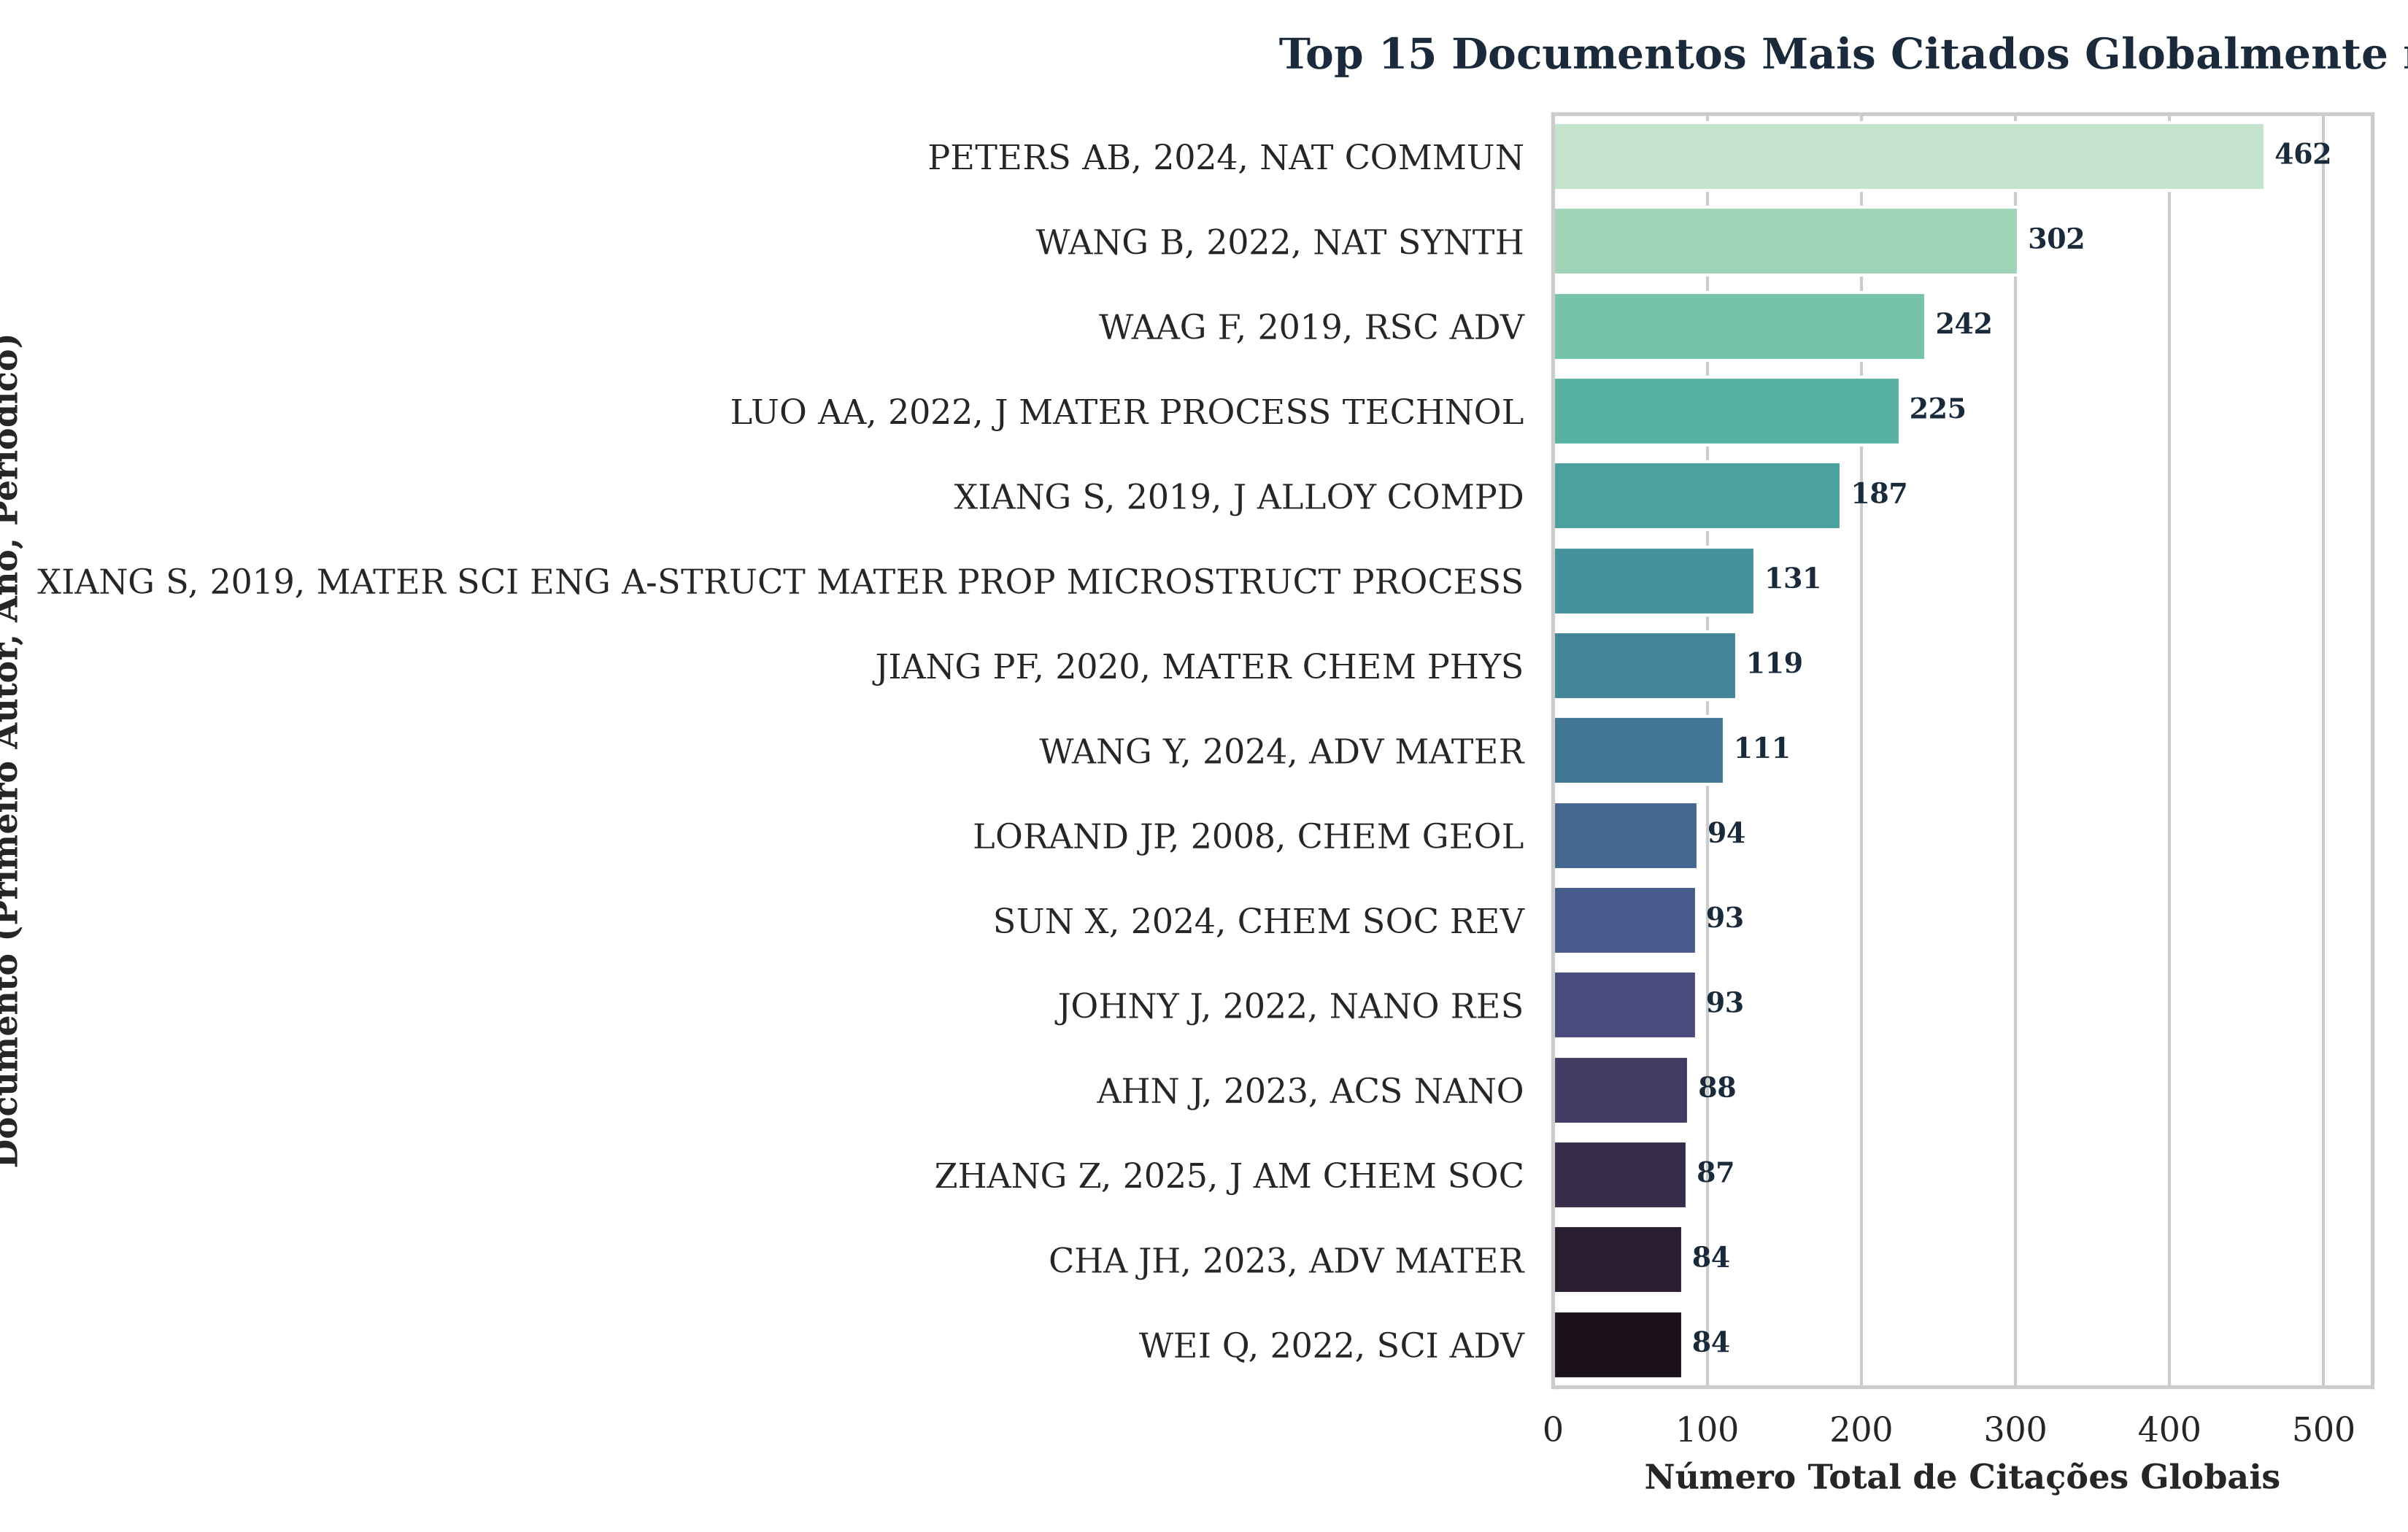
\includegraphics[width=0.85\textwidth]{figuras/most_global_cited_documents.png}
\legend{Fonte: Elaborado pelos autores (2026), a partir de dados da \emph{Web of Science}.}
\end{figure}

\begin{table}[!htbp]
\centering
\caption{Os 10 Artigos Mais Citados Globalmente no Corpus Atualizado}\label{tab:top_glob_docs}
\footnotesize
\begin{tabularx}{\textwidth}{l>{\raggedright\arraybackslash}Xlcc}
\toprule
\textbf{Autor e Ano} & \textbf{Título do Estudo} & \textbf{Periódico} & \textbf{Cit.} & \textbf{Cit./Ano} \\
\midrule
PETERS AB (2024) & Materials design for hypersonics & \emph{Nat. Commun.} & 462 & 154,00 \\
WANG B (2022) & General synthesis of HEA and ceramic nanoparticles & \emph{Nat. Synth.} & 302 & 60,40 \\
WAAG F (2019) & Kinetically-controlled laser-synthesis of colloidal HEAs & \emph{RSC Adv.} & 242 & 30,20 \\
LUO AA (2022) & Alloy development and process innovations for light metals & \emph{J. Mater. Process. Technol.} & 225 & 45,00 \\
XIANG S (2019) & Microstructures and mechanical properties of CrMnFeCoNi & \emph{J. Alloys Compd.} & 187 & 23,40 \\
XIANG S (2019) & Effects of process parameters on tensile properties of LMD & \emph{Mater. Sci. Eng. A} & 131 & 16,40 \\
JIANG PF (2020) & Fabrication and wear behavior of TiC reinforced HEA coatings & \emph{Mater. Chem. Phys.} & 119 & 17,00 \\
WANG Y (2024) & Self-Encapsulation of HEA Nanoparticles in Wood & \emph{Adv. Mater.} & 111 & 37,00 \\
LORAND JP (2008) & Abundance and distribution of PGE in orogenic lherzolites & \emph{Chem. Geol.} & 94 & 4,90 \\
SUN X (2024) & Synthesis of metallic high-entropy alloy nanoparticles & \emph{Chem. Soc. Rev.} & 93 & 31,00 \\
\bottomrule
\end{tabularx}
\legend{Fonte: Elaborado pelos autores (2026), com base em dados da \emph{Web of Science}.}
\end{table}

\begin{figure}[!htbp]
\centering
\caption{Obras fundamentais mais citadas localmente pelo corpus de 192 documentos.}\label{fig:local_cited}
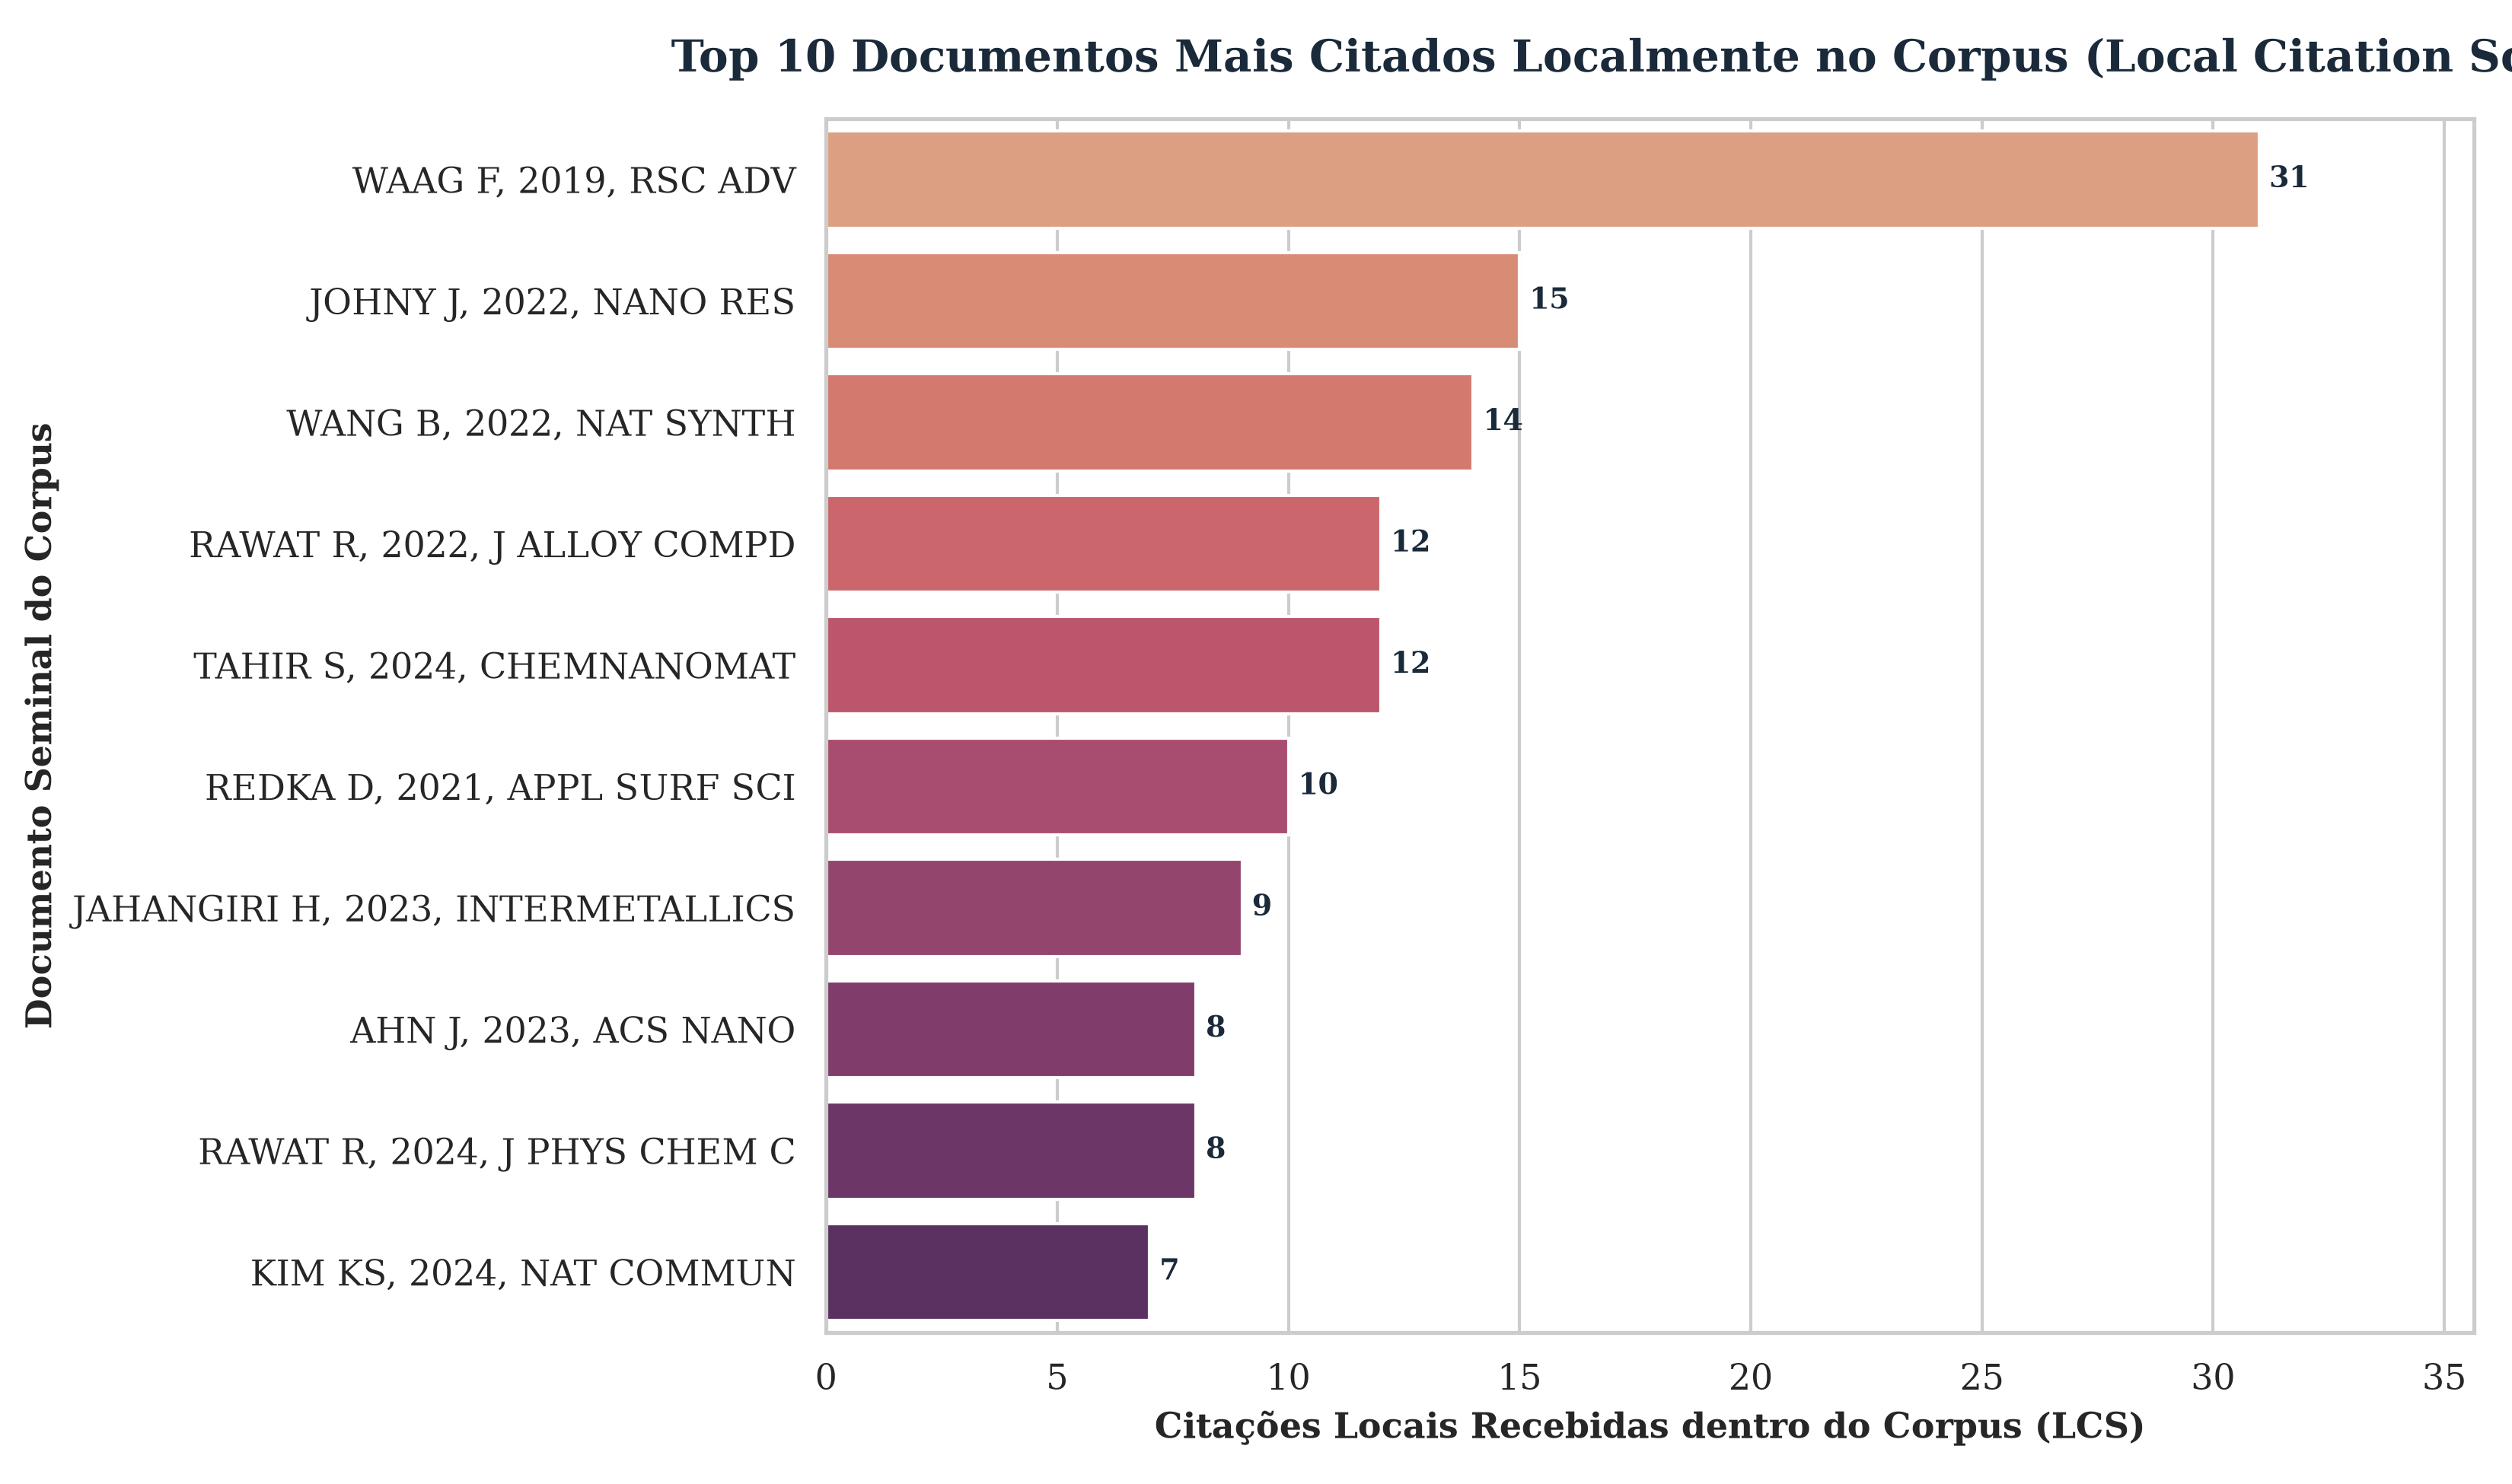
\includegraphics[width=0.85\textwidth]{figuras/most_local_cited_documents.png}
\legend{Fonte: Elaborado pelos autores (2026), a partir de dados da \emph{Web of Science}.}
\end{figure}

\subsection{A Espinha Dorsal Intelectual: De Yeh e Cantor às Ligas Refratárias}\label{a-espinha-dorsal-intelectual-de-yeh-e-cantor-as-ligas-refratarias}

A análise das citações locais na Figura~\ref{fig:local_cited} e nas referências históricas do corpus demonstra a dependência teórico-conceitual do campo em relação a pilares seminais. De um lado, as investigações de Jien-Wei Yeh et al. (2004) e Brian Cantor et al. (2004) romperam com o paradigma clássico do elemento solvente único, formalizando a entropia configuracional ($\Delta S_{\text{conf}} \ge 1{,}5R$) para estabilizar soluções sólidas desordenadas simples (BCC, FCC, HCP) e introduzindo a clássica liga CoCrFeMnNi. De outro lado, Oleg N. Senkov et al. (2010, 2011, 2012, 2018) transpuseram esses princípios termodinâmicos para elementos refratários de ultra-alto ponto de fusão (W, Ta, Mo, Nb, V, Ti, Zr e Hf), demonstrando que sistemas equiatômicos como WNbMoTa e WNbMoTaV retêm limites de escoamento superiores a 400 MPa a 1600 \textdegree{}C, patamar inatingível para superligas à base de níquel.

\subsection{Análise de Palavras-chave e Evolução Temática}\label{sec:analise_palavras_chave}

A análise de palavras-chave permite identificar os principais eixos temáticos e as frentes emergentes da literatura sobre ligas de alta entropia para condições extremas. A partir da frequência e coocorrência dos termos no corpus (Figura~\ref{fig:wordcloud}), a produção científica articula-se em três eixos interdependentes. O primeiro eixo abrange a \textbf{microestrutura e propriedades mecânicas}, com ênfase na estabilização de fases e nos mecanismos de endurecimento (\emph{microstructure}, \emph{yield strength}, \emph{mechanical properties}) para sustentar solicitações mecânicas acima de 1200 \textdegree{}C. O segundo eixo concentra-se na \textbf{resistência ambiental e oxidação}, investigando a degradação sob alta temperatura (\emph{oxidation}, \emph{high-temperature oxidation}) e a inibição da oxidação catastrófica (\emph{pest oxidation}) intrínseca a elementos refratários voláteis. O terceiro eixo focaliza o \textbf{processamento e revestimentos protetores}, impulsionando o desenvolvimento de barreiras térmicas (\emph{coatings}), rotas de metalurgia do pó e manufatura aditiva para integração em componentes aeroespaciais.

\begin{figure}[!htbp]
\centering
\caption{Nuvem de palavras-chave evidenciando os termos de maior frequência no corpus.}\label{fig:wordcloud}
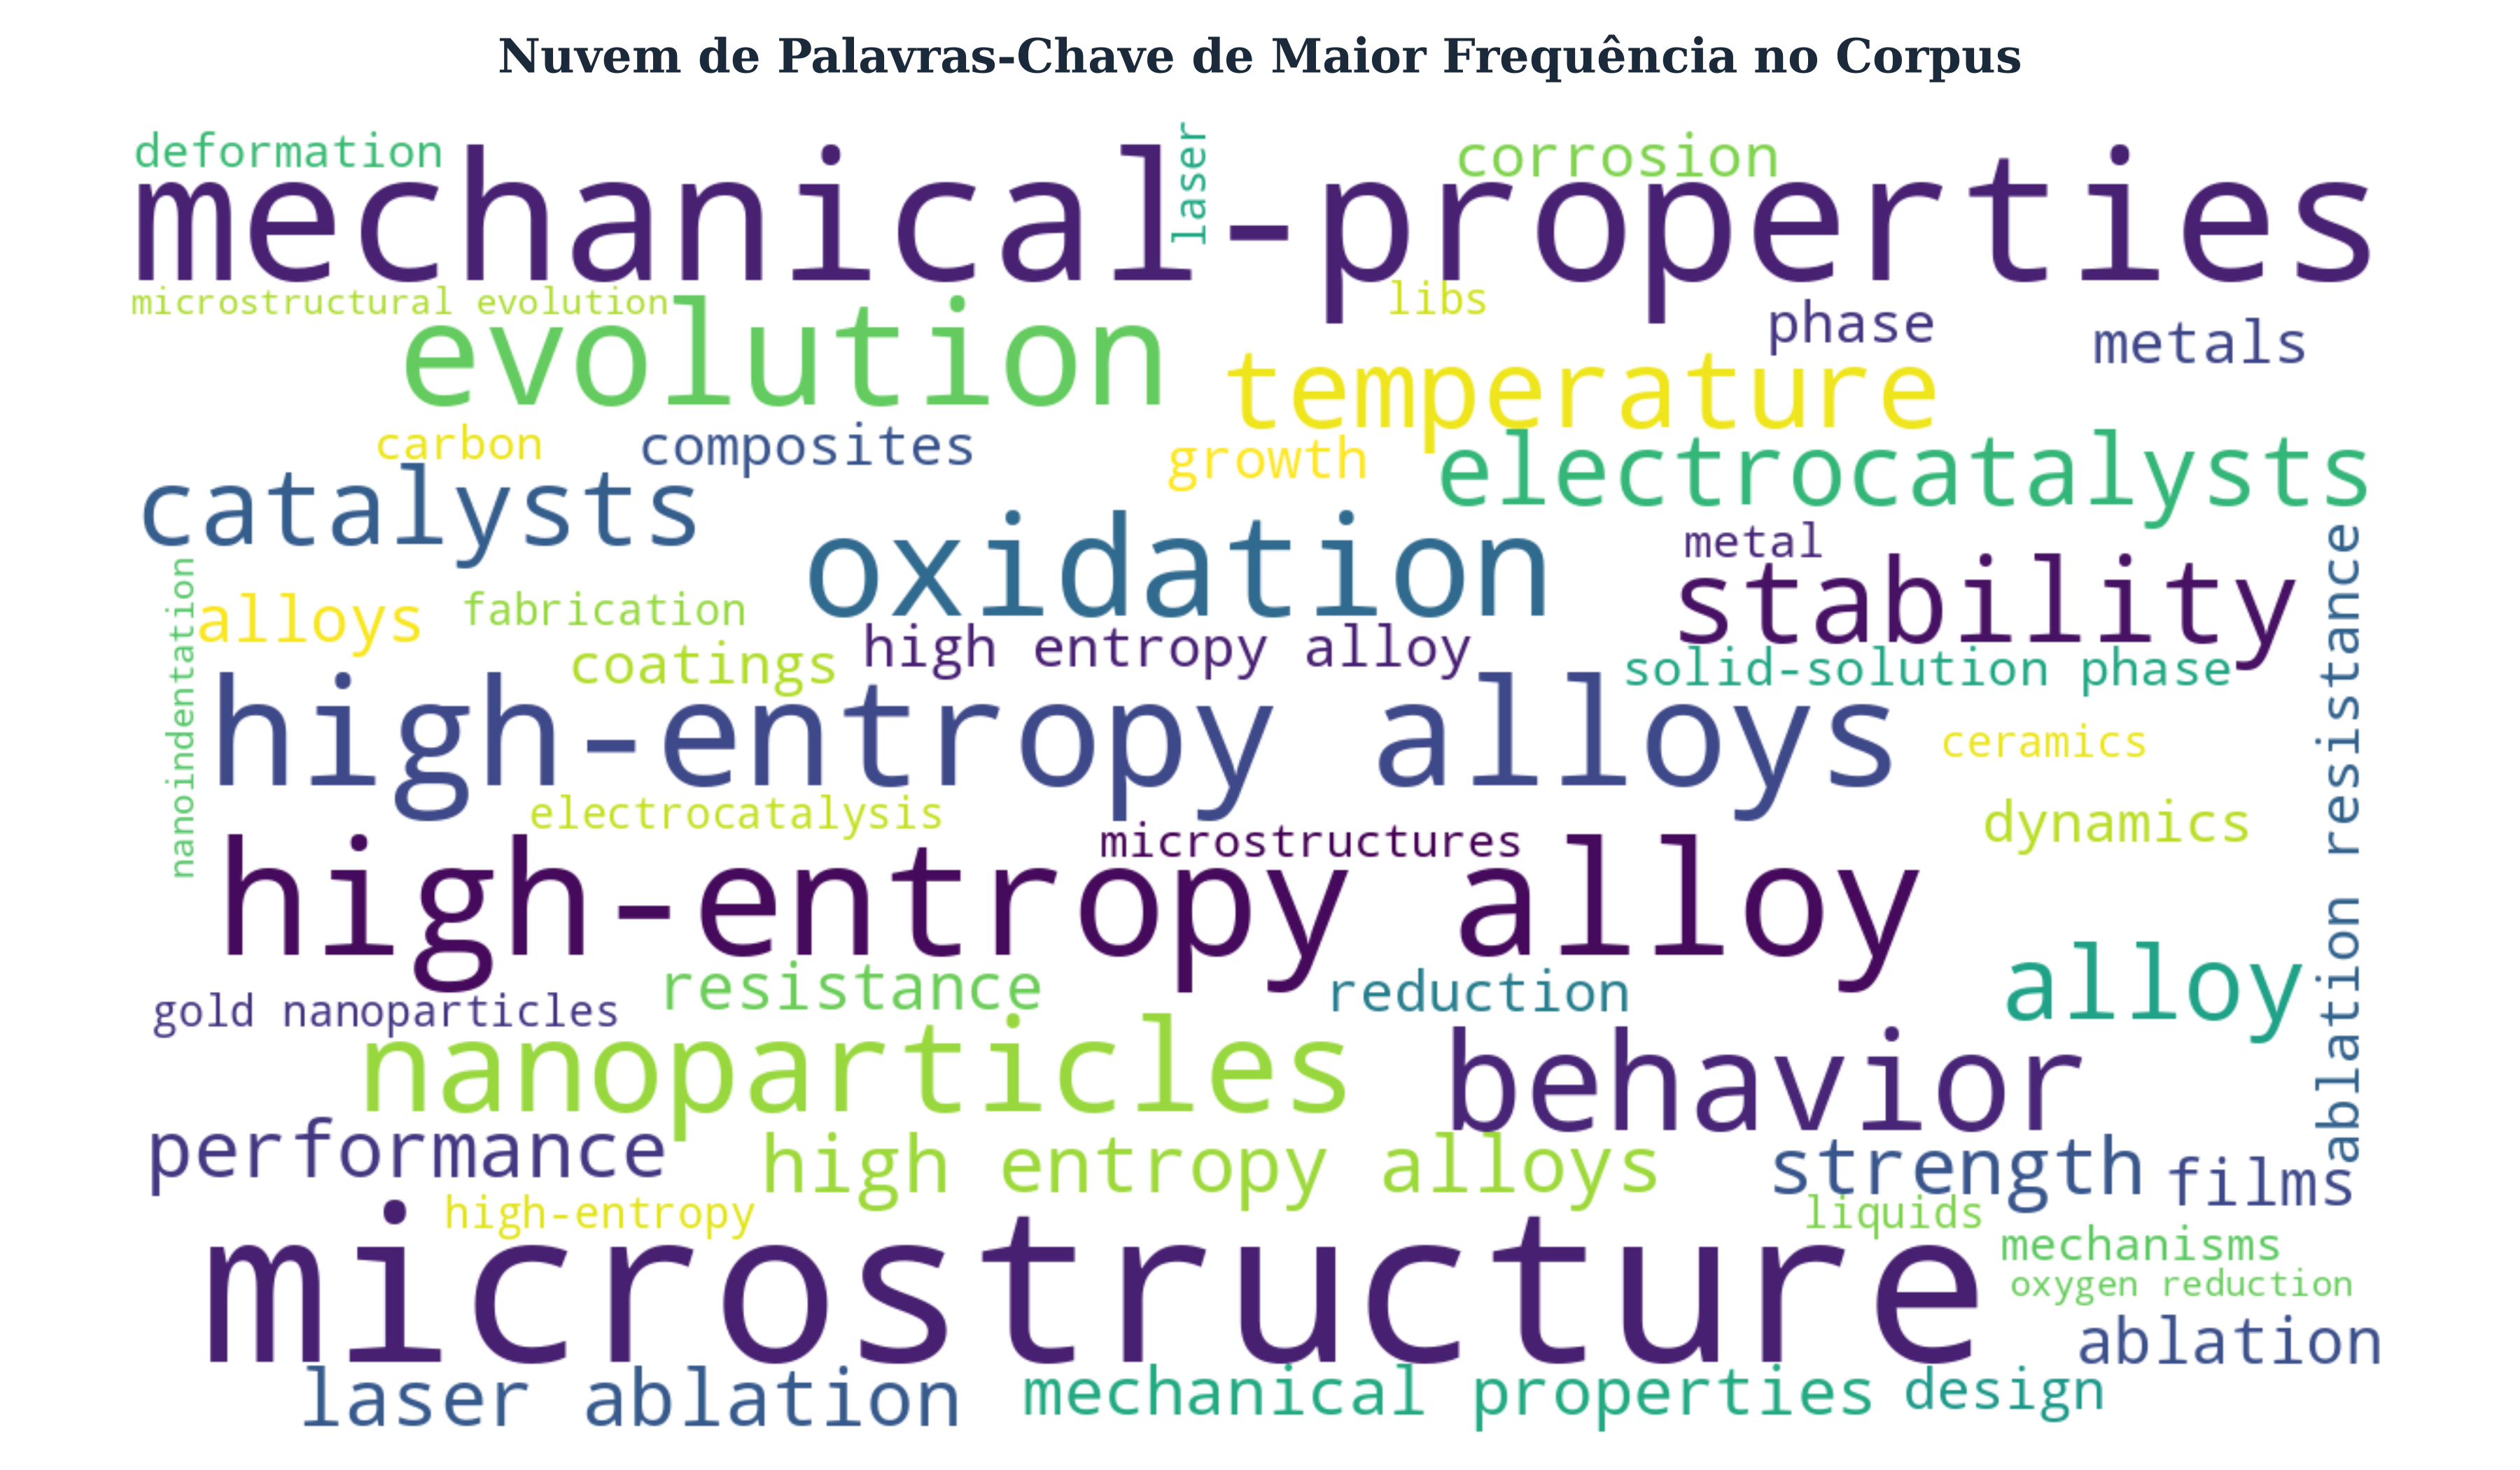
\includegraphics[width=0.85\textwidth]{figuras/wordcloud.png}
\legend{Fonte: Elaborado pelos autores (2026), a partir de dados da \emph{Web of Science}.}
\end{figure}

\begin{figure}[!htbp]
\centering
\caption{Evolução temporal das palavras-chave e tópicos de pesquisa no período 2013--2026.}\label{fig:trend_topics}
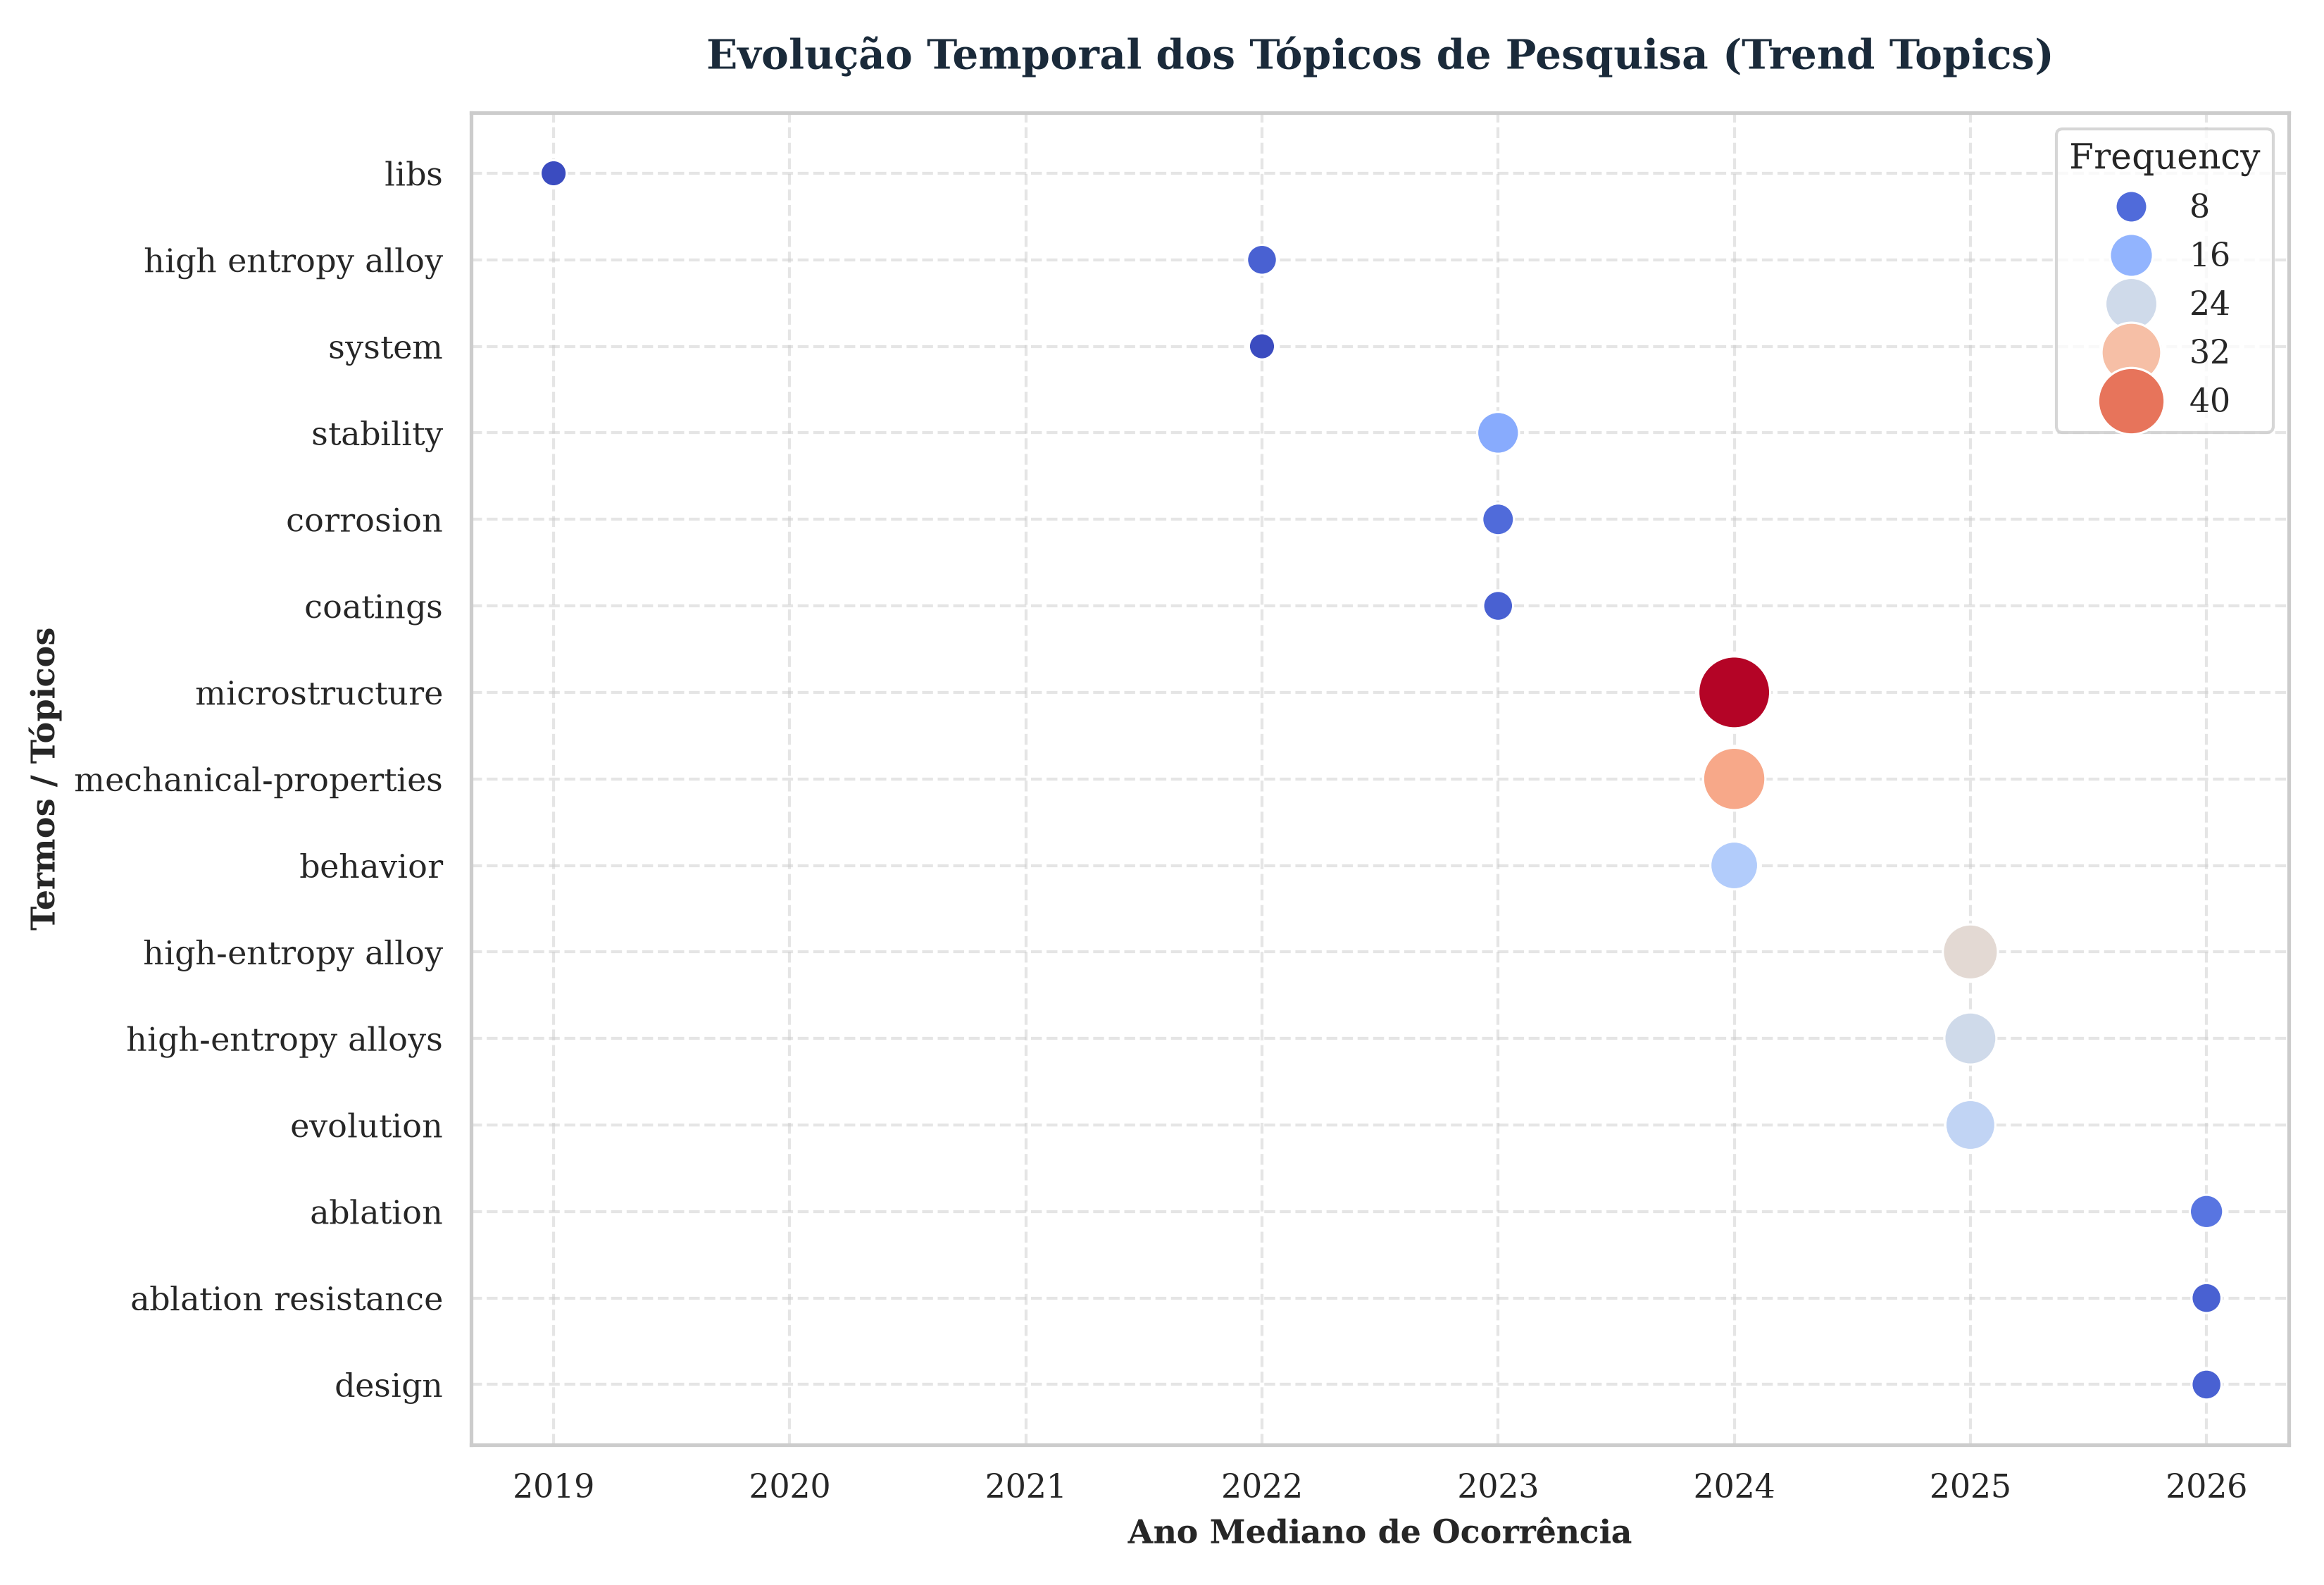
\includegraphics[width=0.85\textwidth]{figuras/trend_topics.png}
\legend{Fonte: Elaborado pelos autores (2026), a partir de dados da \emph{Web of Science}.}
\end{figure}

A análise temporal dos tópicos de pesquisa (Figura~\ref{fig:trend_topics}) evidencia a maturidade gradual da área. Nos primeiros anos (2013--2018), as publicações concentravam-se na caracterização básica de microestrutura, dureza e comportamento em compressão. A partir de 2019, observa-se uma transição nítida em direção à engenharia de ligas aplicadas, destacando-se temas como cinética de oxidação em temperaturas ultra-altas, revestimentos protetores contra ablação e, mais recentemente (2023--2026), o emprego de manufatura aditiva e ferramentas computacionais (CALPHAD e aprendizado de máquina) para aceleração do design composicional.

\subsection{Redes de Cocitação e Acoplamento Bibliográfico}\label{redes-de-cocitacao-e-acoplamento-bibliografico}

A investigação relacional profunda (\emph{Co-citation Network}) confirma a força gravitacional dos fundadores da área. A análise visual de cocitação (referências antigas frequentemente citadas de forma conjunta) atesta que os estudos seminais de Yeh e Cantor (2004) constituem um agrupamento central indissociável dos trabalhos basilares de Senkov (2010), comprovando que a academia percebe as ligas refratárias (RHEAs) como uma extensão ininterrupta e direta do marco termodinâmico de 2004. Por sua vez, o acoplamento bibliográfico (\emph{Bibliographic Coupling}), que agrupa as publicações atuais do corpus que compartilham o mesmo referencial, revela as atuais ``ilhas'' de pesquisa. Identifica-se uma frente focada agressivamente na mitigação de corrosão por meio de \emph{coatings} funcionais protetores e uma frente paralela, frequentemente oriunda do cenário europeu, baseada na predição exaustiva de estabilidade de fases por meio do método CALPHAD.



\subsection{Rede de Coocorrência Institucional e Geopolítica}\label{rede-de-coocorrencia-institucional-e-geopolitica}

O exame das macro-colaborações institucionais delineia a geopolítica da tecnologia de materiais. Enquanto os grafos de colaboração país-a-país indicam a China como a maior produtora em volume bruto, observam-se padrões frequentemente endógenos, onde instituições chinesas colaboram de forma massiva, porém domesticamente (como as conexões fortes entre HIT e Taiyuan). Em contrapartida, polos situados na Alemanha, nos Estados Unidos e na Inglaterra exibem altíssimos níveis de centralidade de intermediação (\emph{betweenness centrality}), operando como os nós conectores essenciais que distribuem o conhecimento ao redor do globo, tecendo redes complexas de transferência e validação de tecnologias para resistência termomecânica.

\subsection{Perspectivas Futuras: Aprendizado de Máquina e Intersticiais}\label{perspectivas-futuras-aprendizado-de-maquina-e-intersticiais}

Os desenvolvimentos recentes registrados na parcela final do corpus (2024--2026) apontam para metodologias emergentes, como a \textbf{Simbiose Machine Learning -- CALPHAD}, acelerando a previsão composicional termodinâmica em bancos de dados ab initio. Em suma, a expansão do corpus bibliométrico comprova que as Ligas de Alta Entropia Refratárias se consolidaram como a plataforma de materiais estruturais definitiva do século XXI.
